\documentclass[12pt]{ociamthesis}  % default square logo 
%\documentclass[12pt,beltcrest]{ociamthesis} % use old belt crest logo
%\documentclass[12pt,shieldcrest]{ociamthesis} % use older shield crest logo

%load any additional packages
\usepackage{amssymb}
\usepackage{amsmath}
\usepackage{amsthm}
\usepackage{listings, multicol}
\usepackage{xcolor, graphicx}
\usepackage{geometry}
\usepackage{algorithm}
\usepackage{algorithmicx}
\usepackage{algpseudocode}
\usepackage{booktabs}
\usepackage{caption, subcaption}
\usepackage[inline]{enumitem}
\usepackage{qtree}
\usepackage{hyperref}
\usepackage{tablefootnote}


%input macros (i.e. write your own macros file called mymacros.tex 
%and uncomment the next line)
\definecolor{c_non}{RGB}{121, 133, 155}
\definecolor{c_sin}{RGB}{247, 141, 184}
\definecolor{c_mul}{RGB}{255, 204, 102}

\definecolor{dkgreen}{rgb}{0,0.6,0}
\definecolor{gray}{rgb}{0.5,0.5,0.5}
\definecolor{mauve}{rgb}{0.58,0,0.82}
\lstset{frame=tb,
  language=python,
  aboveskip=1mm,
  belowskip=1mm,
  captionpos=b,
  showstringspaces=false,
  columns=flexible,
  basicstyle={\footnotesize\ttfamily},
  numbers= left,
  numbersep=5pt,
  numberstyle=\footnotesize\ttfamily\color{gray},
  keywordstyle=\color{blue},
  commentstyle=\color{dkgreen},
  stringstyle=\color{mauve},
  frame=single,
  breaklines=true,
  breakatwhitespace=true
  tabsize=2,
  xleftmargin=\parindent,
  emptylines = *0,
}
\newcommand{\code}[1]{\lstinline|#1|}
\renewcommand{\lstlistingname}{Code}

\theoremstyle{defn}
\newtheorem{defn}{Definition}[chapter]
\newtheorem{emp}{Example}[chapter]

\newcommand{\bv}[1]{\boldsymbol{#1}}

%\include{mymacros}

\title{Ontology-based Visual Analytics \\[1ex]     %your thesis title,
        For Text Analysis}   %note \\[1ex] is a line break in the title

\author{Tianwei Dong}             %your name
\college{Green Templeton College}  %your college

%\renewcommand{\submittedtext}{change the default text here if needed}
\degree{Master in Computer Science}     %the degree
\degreedate{Trinity 2015}         %the degree date

%end the preamble and start the document
\begin{document}

%this baselineskip gives sufficient line spacing for an examiner to easily
%markup the thesis with comments
\baselineskip=18pt plus1pt

%set the number of sectioning levels that get number and appear in the contents
\setcounter{secnumdepth}{3}
\setcounter{tocdepth}{3}


\maketitle                  % create a title page from the preamble info
\begin{dedication}
This thesis is dedicated to my dear parents\\
  Haibo Dong and Aimin Lu
 \\
for their always encouragement and support\\
\end{dedication}        % include a dedication.tex file
\begin{acknowledgements}
I would like to give my deepest gratitude to my project supervisor Prof. Min Chen, who offered me great help and guidance throughout the entire project. Every time I have a problem, he always explain to me patiently and support me all the time.

I would also like to express my gratefulness to my lecturers Prof. James Worrell, Dr. Andrew Ker, Prof. Gavin Lowe, Prof. Stephen Pulman and Prof. Nando de Freitas. Thank them for taught me knowledges in many different areas and trained me necessary skills for completing this project.

Meanwhile, I really appreciate my dear family and friends. It's they who gave me long-term support and assistance in this hardworking and fulfilling year in Oxford. Finally, I want to thank myself. For so many years, harbouring the faith of developing elite into a habit, I am always challenging and beyond myself to realise my dream. Hope I won't forget my initial determination and keep going.
\end{acknowledgements}   % include an acknowledgements.tex file
\begin{abstract}
As the development of Internet, the total amount of data is exponentially increasing. However, the Semantic Web has not been mature, so the implied data of webpages in the traditional World Wide Web cannot be presented in a structured way. Therefore, it appears particularly important to filtering out the target webpage we need and extracting structured information among billions of webpages. 

This project uses the seminar announcement webpages in University of Oxford as a case study and gives a new pipeline to implement the solution. This solution is based on Ontologies and combined the techniques of Machine Learning and Visual Analytics to web data analysis and extraction. We implemented an intelligent crawler to get all the webpages on the University of Oxford's website. An active training classifier is used to filter out seminar announcement pages among them. Users can make correction through visual analytics to interact with the classifier. Then, we implemented a semi-automatic information extraction system. With the help of extraction ontology, users can use visual analytics to easily extract target information. Finally, a well designed visualisation is used to display the extracted seminar announcements, which makes the solution more complete and more usable. Furthermore, the introduction of Ontologies improves the system's ability to extend and migrate.

We got satisfying test results in our experiment as well. Though there is no ready-made dataset, we created one by ourselves with manual classification. Our filter reached a rate of 85\% correctness.

Generally speaking, for text analysis in this information explosion era, this kind of solution provides us a new entry point.

\end{abstract}
          % include the abstract

\begin{romanpages}          % start roman page numbering
\tableofcontents            % generate and include a table of contents
\listoffigures              % generate and include a list of figures
\end{romanpages}            % end roman page numbering

%now include the files of latex for each of the chapters etc
\chapter{Introduction}\label{chapter:intro}
\section{Problem}
Nowadays, data in the internet has gone from scarce to superabundant. This brings us huge new advantages, but also challenges\cite{1_the_economist_2010}. The cyber world contains a large amount of digital data which is constantly changing and getting ever vaster. This makes the raw data widely available everywhere. Meanwhile, the ability of extracting knowledge from the multifarious data becomes desperately needed. ``Researchers need to adapt their institutions and practices in response to torrents of new data — and need to complement smart science with smart searching'', says Nature\cite{Nature:2008jh}.

However, most data on the internet is unstructured, littery and dynamic. Furthermore, they are often wrapped into very different and complicated modes of presentation. When trying to do some automatic search on a specific topic, artificial intelligence will face huge challenges.\\

\noindent There are three scenarios in the real world:
\begin{enumerate}
  \item When a high school student applying for an undergraduate programme, he may need to collect and compare the information of different programmes in different departments and different universities. It includes but not limited to selection criteria, funding, tuition fee and how to apply. However, the introductions to these programmes are on different webpages and share disparate layouts. Thus, the student needs to spend a large amount of time to integrate information about the programmes such as course structure and entry requirement. Furthermore, some information such as course introduction may only exists in PDF files, which makes automatic information extraction even harder.
  \item Another example is looking for the information of current and up-coming art	exhibitions around the country. The exhibitions' open hours and dates could be shown anywhere in diverse forms. For example, on the an exhibition's own website and the various city council's website. It might also have different prices for the tickets, for instance, a person who has a membership may be eligible to enjoy a discount on price. Moreover, the information found might be duplicate, which makes the arrangements of visiting art exhibitions even harder.
  \item Looking up research papers is also an example. When doing literature review, a researcher is usually required to loop up to a large amount of research papers. Nowadays, most of the recent papers could be found online. However, the research papers appear on various websites and are often in PDF format. And one research paper may exists on many different websites. Though based information of these paper are structured, they may have very different webpage layouts. Thus, it is difficult that we build a large database to manage the information and make it convenient for researchers to use.
\end{enumerate}

Hence, this kind of problems have been hard to solve so far. It is mainly because that the semantic web is still not mature and web is based on normal html content. However, these massive layouts make it difficult to integrate structured and logical data. Meanwhile, in order to achieve semi-automation, it is required to pick out the webpage with target information among the large amount of chaotic webpages. Thus, implementing a web page filter is also a big challenge that cannot be ignored.

\section{Case Study: Oxford Seminar Announcements}

The scenarios we stated above might be too large, and the correctness of the result is hard to test. Thus, we decide to choose a relatively small but representative problem in a specific domain for this project. As seminar announcements in the University of Oxford is very typical, we will use it as our case study. Additionally, it is very practical and useful to develop such a system for fellows and students in the University of Oxford.

\begin{figure}[htb!]
	\centering
	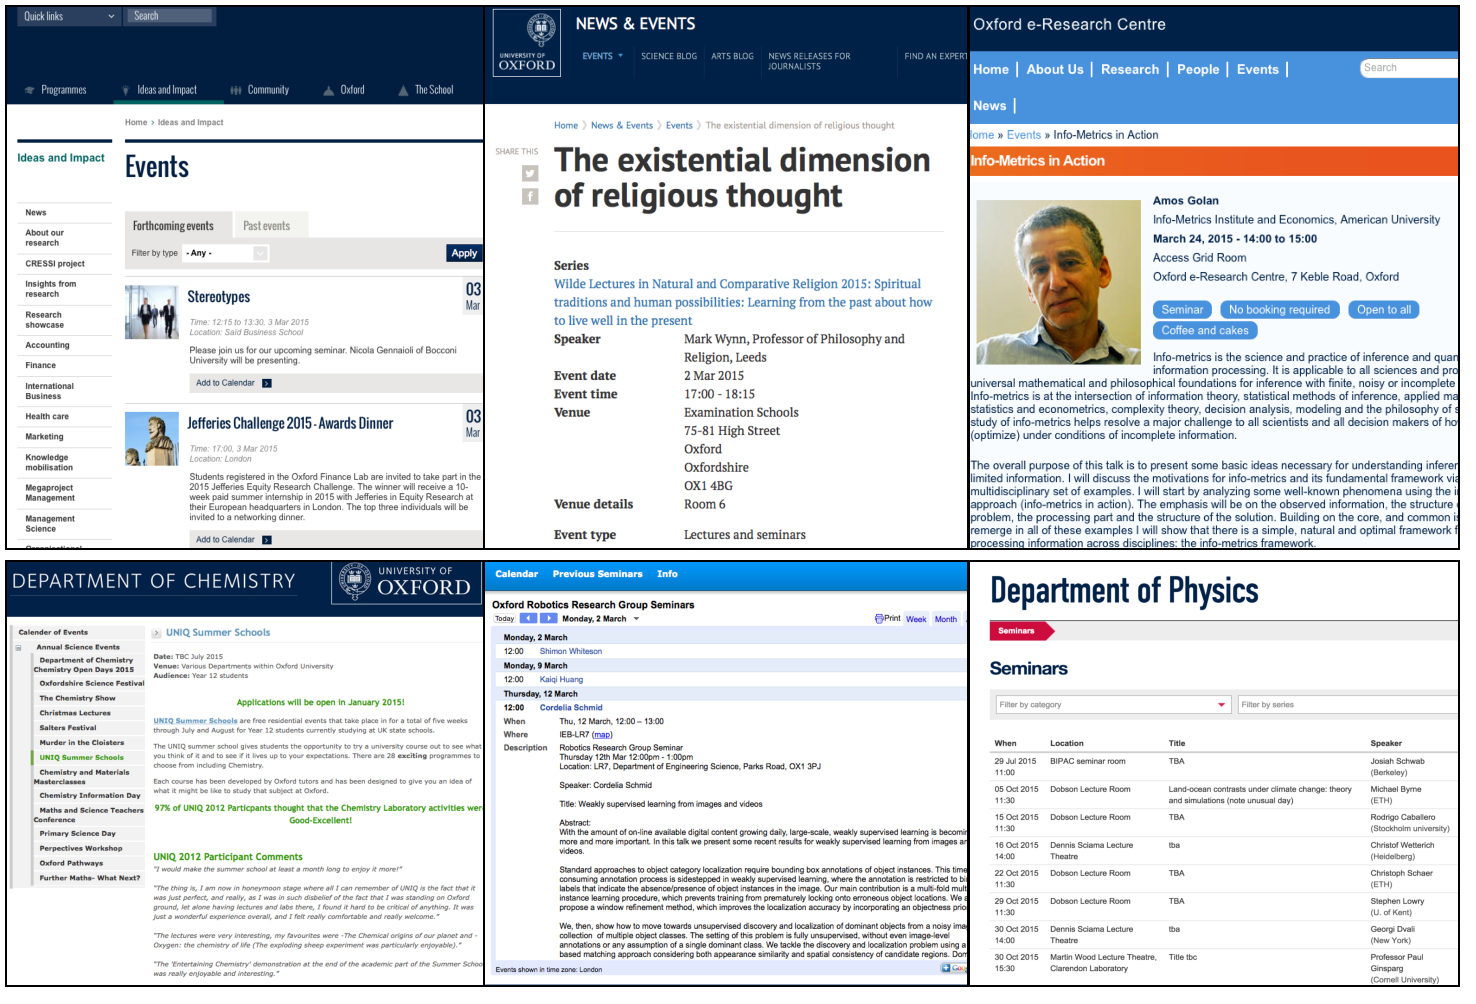
\includegraphics[page=1,width=\textwidth]{images/picture.pdf}
	\caption{Sample Seminar Announcement Pages in University of Oxford Websites}\label{fig:emp:various_layout}
\end{figure}

There are numerous seminar announcements in University of Oxford each week, and they are structured very differently and exhibits in various forms(as shown in Figure \ref{fig:emp:various_layout}). The majority of 395 departments and 38 colleges have their own website\footnote{data is obtained from University of Oxford official website}, and most of them has its own way to display seminar information. A rough statistics shows that currently there are approximately 2000 seminars taking place in Oxford every month\footnote{data is estimated by the google search result}. Filtering out the related web pages, extracting required data and visualising seminar information from such a huge amount of web pages is a very difficult and complicated process. And seminar information updates frequently, which makes demands on high efficiency. It can hardly be done by human beings manually. 

Therefore, the system we developed here should be capable of filtering seminar announcement pages from the given domain, dynamically collecting seminar information each week throughout the billions of Oxford web pages and present them in numerous visualisation forms.

\section{Aims and Objectives}
The purpose of this project is to design and develop an semi-automatic system to solve such complex problem. The system covers the entire process from data collecting at the beginning and data presentation at last. It needs to do web page classification based on machine learning and human interaction. Meanwhile, it is able to capture information and generate corresponding tabular data from the given domains, and provide a visualisation to show the result knowledge for the end users by using state of art technologies. Both web page classification and information extraction are completed with the help of visual analytics. In general, it is the process of ontology-based visual analytics for text analysis.

In particular, considering our study case, the entire project is required to achieve the following objectives:
\begin{itemize}
	\item Implement an intelligent crawler to conduct web crawling in the University of Oxford's website;
	\item Design and implement an ontology-based automatic web page filter to pick out all the target webpages that contain seminar announcement;
	\item Create data sets for seminar announcement pages;\footnote{There is no existing data set for seminar announcement pages, we should create it by ourself manually.}
	\item Design and conduct experiments to test the web page classification above by using the data sets;
	\item Design and implement a semi-automatic solution to extract the seminar announcement information from the target webpages under the assistance which combining ontology and visual analytics.
	\item Design and implement a visualisation to present a large number of seminar announcements;
	\item Create a pipeline and implement a complete and feasible system to combine all the function above together to form a systematic solution.
\end{itemize}

\section{Setting and Assumption}
\begin{enumerate}
	\item Domain\\
	This project will constraint the targets within the domain of \code{ox.ac.uk}, i.e. all webpages in this domain will be covered in this project.
	\item Target Entity\\
	Seminar announcement information is regarded as the target entity.
	A seminar announcement page is a web page that contains at least one announcement for a seminar.
	According to the Merriam-Webster Dictionary, a `seminar' is `
	\begin{enumerate*}[label=\textit{(\arabic*)}]
		\item \textit{a meeting in which you receive information on and training in a particular subject;}
		\item \textit{a class offered to a small group of students at a college or university}
	\end{enumerate*}'.
	An `announcement' is `\textit{a written or spoken statement that tells people about something: public or formal words that announce something}'\cite{merriam2004merriam}.
	
	Therefore, a seminar announcement in Oxford is a statement which tells people about information related to a short training or meeting in the University of Oxford. It must contain at least the following facts related to a seminar: 
	\begin{center}
		date, time, location, subject, speaker
	\end{center}
	It may also contain information about:
	\begin{center}
		target audience, abstract of seminar, short introduction of speaker, \\
		how to book, organiser, seminar frequency
	\end{center}	
	
	\item Attribute\\
	Based on the study on a large number of seminar announcement pages on the Oxford websites, we decided to select the following attributes of seminar announcement in research:
	\begin{center}
		date, time, title, location, speaker, abstract		
	\end{center}
	It contains format information including string, time and date.
	\item Dynamic Page Techniques\\
	Here, we do not consider the various webpage structures generated by the front-end dynamic page technologies such as Ajax, AngularJS\cite{mesbah2012crawling, grant2014basics}. Because in order to construct these webpages, we need to implement a browser kernel to parse and execute javascript. However, this project focuses on using ontologies and visual analytics to do semi-automatic webpage classification and information extraction. As time is limited, we decide to ignore these kinds of dynamic pages.
\end{enumerate}


\section{Dissertation Structure}
In this dissertation, we will first give a brief introduction to the problem we are going to solve, especially why we have this problem and what is our study case.

Next, we will give the background study and literature review for the project in chapter \ref{chapter:bg}. First of all, we will briefly introduce the wide background knowledge related to our solution. Secondly, there will be a short discussion about the related research and solutions so far.

In chapter \ref{chapter:solution}, we will state a formal setting of the problem we are facing and give an overview of the solution. The key issues and main challenges will be described here. There will also be an explanation to the whole solution pipeline of this ontology-based visual analytics for text analysis.

In the following chapter \ref{chapter:clf} and chapter \ref{chapter:ie}, an explanation of the core parts in our solution, webpage classification and information extraction, will be delivered in details. It helps with showing the readers what are the advantages of this solution.

Last but not least, there will be a critical thinking part about further study and conclusion. We will give the adaptability of the solution and some possible applications in other areas.

\chapter{Background}\label{chapter:bg}
The problem stated above is extremely complicated. It is a systematic engineering which involves several involuted and independent research topics, such as webpage classification, information extraction and webpage annotation. In this chapter, a literature review of related research areas will be given at beginning, then we will provide some existing related methods and their disadvantages.

\section{Literature Review}
\subsection{Semantic Web}
20 years ago, the World Wide Web was invented to be used as a web of documents. However, as the change of the time, the data inside the documents are receiving more attentions. The purpose of the Semantic Web is building a kind of web which connecting all the data in a relational structure rather than simply a pile of unrelated documents\cite{shadbolt2006semantic}. The occurrence of Semantic Web makes the human be able to focus on the raw data instead of the mess and various web page documents\cite{berners2001semantic,shadbolt2006semantic}.

The semantic web is now regarded as an extension of the Web through standards by the World Wide Web Consortium (W3C). This is considered as next generation of web by Tim Berners-Lee, the inventor of the Semantic Web. According to the W3C and Tim Berners-Lee, "The Semantic Web provides a common framework that allows data to be shared and reused across application, enterprise, and community boundaries". It promotes common data formats and exchange protocols on the Web, most fundamentally the Resource Description Framework (RDF)\cite{berners2001semantic}. 

According to Berners-Lee, the Semantic Web normally have the following components: data resources, links among data and relative tools\cite{berners1998semantic}. Compared with the Semantic Web, the traditional World Wide Web do not have a mechanism to process data. It is the obstacle when transferring from traditional Web Wide Web to Semantic Web era. Today, most of the content on the internet has not been structured into semantic information. Meanwhile, according to Marshall and Shipman, much knowledge's tacit and changing nature  adds to the knowledge engineering problem, and also limits the applicability of the Semantic Web to specific domains\cite{marshall2003semantic}. That is where our project becomes meaningful. 

On the other hand, the purpose of building semantic web is making the linked data on the internet be easily extractable. If we are able to develop a technique which can extract required information in the webpage automatically, the problem will be solved.

\subsection{Ontology}
The word ``ontology'' is used in different communities with different meanings. Here we are talking about Ontology in the knowledge engineering community. At early stages, the computational ontologies are defined as ``explicit specifications of conceptualisations''. Guarino1, Oberle and Staab gave us a clarified definition: they are a method of modelling the structure of a system by means of its entities and the relationships between the entities. Formally, they are considered as ``concepts''(i.e. taxonomy) and ``relations''\cite{guarino2009ontology}.

An ontology is a formal definition and naming of the types, properties and interrelationships of the entities that fundamentally exist for a particular domain of discourse. It compartmentalises the variables needed for some set of computations and establishes the relationships between them\cite{Gruber:1993:TAP:173743.173747}. It could be considered as a graph of relationships between entities and a kind of specification mechanism\cite{maedche2002ontology}.

Currently, there exists many ontology representation languages, including, but not limited to: Description Logics(DL), Resource Description Framework(RDF) and Web Ontology Language(OWL). Meanwhile, there are also many infrastructures for ontologies, such as RDF storage and retrieval systems, tableau-based reasoning and ontology mapping\cite{staab2013handbook}.

\begin{enumerate}
\item \textbf{Web Ontology Language(OWL)}\\
OWL is a language which describes the relation of knowledge in the Web, especially Semantic Web. It has several different sublanguages: OWL Lite, OWL DL and OWL Full\cite{maedche2002ontology}.

\item \textbf{Domain Ontology}\\
A domain ontology aims to eliminate (or reduce) the terminological and conceptual confusion among the members of a virtual community of users who need to share a variety of information\cite{Navigli:2004:LDO:1105710.1105712}.

\item \textbf{Ontology Mapping}\\
Ontology mapping provides a common layer where several ontologies could be accessed and semantically exchange information\cite{Kalfoglou:2003:OMS:975027.975028}.
\end{enumerate}

\subsection{Webpage Classification}
Web page classification is usually a system that automatically classifies web pages into meaningful categories. There are two types of web page classifications: genre based and subject based classifications. 

Classification is normally conducted as a supervised learning problem \cite{joachims1997webwatcher}. A set of pre-labeled data is used to train the classifier model, then apply this model to label the other data which need be classified. For information retrieval tasks, classification of Web content is regarded as an important phase.

It uses the state of the art techniques and subsystems to develop automatic web page classification systems, including web page representations, dimensionality reductions, Web page classifiers, and evaluation of Web page classifiers. This kind of systems are essential tools for Web Mining as well as the future of the Semantic Web\cite{choi2005web}.

The classifier for Web page classifiation should concern about more features than text classification, because Web page is a kind of rich text \cite{Qi:2009:WPC:1459352.1459357,joachims1997webwatcher}. Some related attributes, such as HTML tags and URLs, can be involved in the classification process. We will give a brief introduction on some Web page classification techniques in Section \ref{sec:related_methods}.

\subsection{Information Extraction}
Information extraction means to extract the structured data out from unstructured or semi-structured data automatically, and then transform it into a machine readable format\cite{Cowie:1996:IE:234173.234209}. Typical subtasks of information extraction that we are going to focus on includes: named entity extraction, semi-structured information extraction, and language and vocabulary analysis.

There are two types of information extraction tools\cite{chang2006survey}: 
	\begin{enumerate*}[label=\textit{(\arabic*)}]
		\item finite-state tools, which is based on automata and fixed rules. For example, STALKER and WIEN.
		\item relational learning tools, which is based on logic programs likes Prolog. For example, Pinocchio, SRV and WebFoot\cite{soderland1997learning,ciravegna2000learning}.
	\end{enumerate*}

In terms of traditional Web pages, as they are designed differently and do not use structured data schema(such as RDFS), it is very complex and time consuming if we want to automatically extract the data in a web page which is related to the required target. There are also several existing information extraction techniques to solve these problems. They will be introduced in Section \ref{sec:related_methods}.

\subsection{Webpage Annotation}
Long time ago, human beings knew how to use marginal annotations on some part of a text for highlighting purpose. Text Annotation uses highlights, underlines, footnotes and tags etc. as tools to attract reader's attention\cite{shabajee2003annotation}. Web-based text annotation systems allow users to produce marginal annotations with threaded discussions through a simple web browser. Modern web-based text annotation system is a collaborative software that is able to realise text editing and versioning functionality, as well as annotation and commenting interfaces\cite{lebow2009new}. 

A web annotation refers to an online system which is linked to an Internet resource, mostly a web page. Having such a system, a user do not need to alter the resource itself while adding, modifying or removing information from a web resource. It is similar to a layer, usually visible, covering the existing resource. Other users, who share the same annotation system, also have access to it.

Web annotation can be used as a collaborative tool, such as discussing the contents of a certain resource. It is also able to to quantify transient relationships between information fragments.\\

Besides the above three core topics, there are also some relevant topics and techniques involved in the project. Before we move to current exist methods, we are going to give a brief introduction to the related background knowledge here.

\subsection{Visual Analytics}
Visual analytics is an outgrowth of information visualisation and scientific visualisation that focuses on analytical reasoning with interactions based on visual interfaces\cite{VisualAnalytics2004}. It can attack certain problems which can be made otherwise intractable by their complexity, size and need. It is a combination of both human and machine analysis. Visual analytics promotes science and technology development in terms of data transformation, analytical reasoning, interaction\cite{tory2004human,VisualAnalytics2004,andrienko2007visual}. They are also representations for analytic reporting, computation and visualisation, and technology transition\cite{VisualAnalytics2004}. It is a combination of several scientific and technical communities including computer science, information visualisation, graphic design, interactive design, cognitive and perceptual sciences, and social sciences.

In addition, visual analytics corporates novel computational and theory-based tools into innovative techniques and visual representations to make human-information discourse viable\cite{VisualAnalytics2004}. There are three principles: cognitive, design and perceptual principles. They are used to govern the design of the techniques and tools\cite{VisualAnalytics2004}. One can develop both tactical and strategic visual analytics technologies for threat analysis, prevention, and response upon the reasoning framework which provided by analytical reasoning\cite{tory2004human,VisualAnalytics2004}. It is the core of the analyst's task of applying human judgements to reach conclusions by combining both evidence and assumptions.

We put the most effort on information visualisation. Information visualisation uses visual representations and interaction techniques to represent abstract data, including both numerical and non-numerical data, to reinforce human cognition\cite{andrienko2007visual}.

Furthermore, visual analytics can be used to assist machine learning process. The result could be much more accurate and reader-friendly when combining these two together. Visual analytics makes humans be able to directly take part in the process of machine learning as well as give fast correction to improve the accuracy of machine learning\cite{andrienko2007visual}.



\subsection{Decision Tree}
A decision tree is a tree-like model of decision analysis structure used in decision process\cite{olaru2003complete}. It is a decision support tool. 

In a decision tree, there are three kinds of components: 
\begin{itemize}
  \item \textbf{internal node}: represents a ``test" on an attribute;
  \item \textbf{branch}: represents the outcome of the test
  \item \textbf{leaf node}: represents a classification label
\end{itemize}
Meanwhile, the paths from root to leaf represents the classification rules. Drawn from left to right, a decision tree has only burst nodes but no sink nodes. In other words, a decision tree only splits paths, but never converge paths. Therefore, used manually, they can grow very big and then are often hard to draw fully by hand\cite{olaru2003complete}.

Among decision support tools, decision trees have several advantages\cite{breiman1984classification,quinlan2014c4}:
\begin{itemize}
  \item Simple to understand and interpret. Ordinary people can easily understand a decision tree model after a brief explanation;
  \item Easy to update(optimise) because that it allow human adapted some new scenarios into the model;
  \item It is a white box model;
  \item It will still work when the size of data set is small, and human experts can involved their knowledge and preferences into the decision procedure to improve the performance;
  \item We can involved visual analytics and human interaction, because it can be integrated  with other decision methods.
\end{itemize}

Particularly, decision tree is much more expressive for a semantic project. On the other hand, it conforms the rules and habits how human beings classify webpages, and therefore more intuitive. 

\begin{figure}[htb!]
	\centering
	\Tree
	[.$f_1>3$
     	[.$f_2>0$
     		[.$f_3>5$
     			[.Class3 ]
     			[.Class1 ]
     		]
     		[.Class2 ]
     	]
     	[.$f_3<=8$
     		[.Class1 ]
     		[.Class2 ]
     	]
     ]
	\caption{Example of Decision Tree}\label{fig:emp:dtree}
\end{figure}

\subsection{DOM Tree}
DOM is short for `Document Object Model'. DOM Tree is the method of using DOM to parse HTML webpages and generate HTML tree structure with the corresponding access method. With the help of DOM Tree, we are able to directly operate on every content markups on HTML pages easily. DOM technology uses a very direct and consistent way to do modelling on the HTML file, and thus provides a simple programming interface for access, navigation and operation page. By using DOM, we can easily access and update not only the content, but also the structure of a web page. This technology is promoted by W3C, therefore, most of the browsers will finally support it.

\begin{figure}[htb!]
	\centering
	\Tree
	[.html
     	[.head
     		[.title ]
     		[.meta ]
     	]
     	[.body
     		[.div
     			[.span ]
     			[.p ]
     			[.p ]
     		]
     		[.hr ]
     		[.div ]
     	]
     ]
	\caption{Example of HTML DOM Tree}\label{fig:emp:html_dom}
\end{figure}

\subsection{Multi-agent System}
Multi-agent system can be used to realise the complex functional systems. According to Wooldridge\cite{Wooldridge:2009:IMS:1695886}, ``an agent is a computer system that is capable of independent (autonomous) action on behalf of its user or owner (figuring out what needs to be done to satisfy design objectives, rather than constantly being told).'' A multi-agent system consists of a number of agents that interact with each other. More generally, agents are acting on behalf of users with different motivations and goals\cite{Wooldridge:2009:IMS:1695886}. For the purpose of successful interaction, they are required to have the ability of cooperation, coordination and negotiation with each other, just like people do.

There are several visions for the usage of a multi-agent system. For example, it is time-consuming and tedious to search the Internet for the answer to a specific query. So an idea could easily come up: using a computer program - an internet agent - to do searches for us.

\section{Current Related Methods}\label{sec:related_methods}
Recent decades, there have been some related research and applications in the areas of webpage classification, information extraction and webpage annotation. We will give a brief review of them in chronological order.

\subsection{Webpage Classification}
In 2001, Tsukada, Washio and Motoda tried to automatic Web-page classification based upon machine learning techniques. They proposed methods to generate attributes by using co-occurrence analysis and to automatically classify Web-page through machine learning\cite{tsukada2001automatic}. 

In 2006, Kan and Thi chose to use only the uniform resource locator (URL) to do web page classification. They segment the URL into meaningful chunks and adds component, orthographic and sequential features to model salient patterns\cite{kan2005fast}. Then, in 2009, Qi and Davison raised the idea of using features provided by the interconnected nature of hypertext to do classification\cite{Qi:2009:WPC:1459352.1459357}.

As a probabilistic classifier, Naive Bayes Classifier is the most used classifier in this kind of text classification tasks\cite{cichosznaive}. By calculating the probability that a pattern $p$ is a instance of class $c$ under the data observation $o$(i.e. $\Pr(c\vert p)$), each data entity in the training data set are used to estimate the parameters of the model. When testing, $\Pr(p\vert c)$ denotes the probability that a given data with pattern $p$ belongs to a specific class $c$.

There is also a SVM(Support Vector Machine) based classifiers. Under the fact that SVM have an excellent performance in classification\cite{tong2002support}, it is a idea classifier for Webpage classification with the help of kernel and margin.


\subsection{Information Extraction}
In 1999, Stephen Soderland produced an information extraction application called WHISK which is able to learn text extraction rules automatically to handle semi-structured text styles ranging from highly structured to free text\cite{soderland1999learning}. Meanwhile, Finkel, Grenager, and Manning chose to do extraction by modelling non-local structure instead of the various Markov Models. They use Gibbs Sampling to incorporate non-local structure while preserving tractable inference\cite{finkel2005incorporating}. 

In 2007, Banko, Cafarella and Soderland et al. brought up the concept of Open Information Extraction from the Web. They introduced a new extraction paradigm called Open Information Extraction (OIE), where the system makes a single data-driven pass over its corpus and extracts a large set of relational tuples with no human input. They also gave an example of OIE called TextRunner, in which the tuples are assigned with probabilities and indexed to support extraction via user queries\cite{banko2007open}.

\subsection{Webpage Annotation}
In 2002, Yee implemented a set of hypertext linking features called “CritLink” to enable public annotation on the web\cite{yee2002critlink}. On the same year, Kahan, José, et al. proposed an open RDF infrastructure for shared web annotations. They combined RDF with XPointer, XLink and HTTP to implement a web-based shared annotation system called `Annotea', where annotations are modelled as a class of metadata\cite{kahan2002annotea}.

\section{Weakness}
There are several disadvantages if we use these methods to solve the problem we introduced above.

First of all, these methods heavily bias on pure automation and machine learning. This kinds of practical problem requires an extremely extremely high rate of correctness. For example, fully automatic webpage classification cannot assure even 80\% accuracy by using current technology. However, these existing solutions could not perform very well. Because fully automatic programs are not able to cover all the sub tasks in this project. In other words, no human interaction during the whole process of this job may not applicable at this moment.

Secondly, even if we apply these current solutions to our problem without concerning the accuracy, each solution is only able to solve a small part of this big problem. In addition, each part alone is already been a complex issue. For example, information extraction from unstructured and changing webpages has been a well-known public challenge so far. And this project combines these small parts together to form a semi-automatic system, which makes the problem become even more troublesome and complicated.

Furthermore, most current techniques for information extraction are focusing on dealing with pure text. But in our mission, the targets are webpages instead of text documents. Their methods do not fully consider or use the characteristics of html webpages and http response header. On the other hand, most of today's solutions to this problem are dealing with structured or semi-structured data, whereas most data on the internet is in unstructured layout. This makes the problem becomes exponentially harder to solve.






\chapter{Problem Statement and Solution Overview}\label{chapter:solution}
In this chapter, the formal setting of our case study will be given. We will also demonstrate some key issues and main challenges in this problem. Then we will deliver our pipeline and solution overview for ontology-based visual analytics for text analysis.

\section{Problem Statement}
This project is going to solve the problem of integrating and visualising useful information from a large number of web pages. The biggest challenge of the project is acquiring requisite data from various HTML web pages by using semantics web technologies and transferring the data to the corresponding ontologies for the visualisation. About only a few decades ago, this was considered as an impossible task. Nowadays, with the help of ontologies, automated text processing becomes conceivable\cite{krallinger2012link}.

As we stated above, because of the development of information technology and cyberspace, data is growing exponentially on the internet. A piece of useful information is often mixed with irrelevant data or shown on different web pages redundantly. Meanwhile, the information is presented in a great diversity of ways and thus makes it more difficult for humans to handle and integrate\cite{anantharangachar2013InfoExtraction}. In this chapter, we will firstly using seminar announcement pages in University of Oxford as the example to state the complexity and difficulty of this problem.

First of all, for the purpose of getting all the seminar announcements, it is necessary to crawl all the web pages in the entire website of University of Oxford. However, our research object is information that very sensitive to time, such as seminar announcements. Every hour and every day, numerous seminar announcements webpages are created, updated or deleted. Seizing these changes efficiently and accurately is a big challenge for our system. 

\begin{figure}[htb!]
	\centering
	\includegraphics[page=2,width=\textwidth]{images/picture.pdf}
	\caption{Examples: Target Page and Non-Target Page}\label{fig:emp:target_vs_non}
\end{figure}

\begin{figure}[htbp!]
	\centering
	\includegraphics[page=3,width=0.93\textwidth]{images/picture.pdf}
	\caption{Examples: Various Presentation of Seminar Announcement}\label{fig:emp:various_present}
\end{figure}

Next, how to distinguish between our target webpage(i.e. seminar announcement page) and the large amount of the webpages crawled by the system is still a complex problem. For instance, the two webpage screenshots in Figure \ref{fig:emp:target_vs_non} both contain indicators\footnote{e.g. `\textbf{Date:}',`\textbf{Time:}',`\textbf{When:}'} and entities\footnote{e.g. `Fri, 24 Jul 2015',`10:00',`24th June 2015'} about date and time, name and location information. They also have a great similarity of page layout between each other. Meanwhile, there are many seminar announcements pages with totally different page layouts (such as Figure \ref{fig:emp:various_present}) too. It is extremely hard for a machine to tell the difference and further decide whether they are seminar announcement pages. A machine could make a decision in next to no time but with low accuracy. However, it is easy for a human to judge as long as he understands English, and the result will be much more accurate than a machine.

Despite of this, there are other problems. One of the most troublesome challenges among them is data extraction from natural language and processing the ontology integration automatically\cite{maedche2003bootstrapping}. Although we have confirmed a web page contains seminar information, extracting those information is still not easy. For example, consider these three seminar announcement web pages from different departments (see Figure \ref{fig:emp:various_present}). 

The first screenshot comes from the Mathematical Institute\footnote{ \url{https://www.maths.ox.ac.uk/node/14127} at 01:00, 27th Jul 2015 }. We could see that related information such as `31 August 2015 09:00', `L3' and `Derived structures in geometry and representation theory' are in different grids. But there is no distinct indicator word (such as `Date', `Time' and `Location') to indicates. The second screenshot comes from the the Cyber Security Centre in Department of Computer Science\footnote{ \url{http://www.cs.ox.ac.uk/seminars/1439.html} at 01:00, 27th Jul 2015 }. Information such as time and location are listed corresponding to each indicator. Speaker and title are stated separately in the header. Unlike the previous two, the third screenshot (department of physics)\footnote{ \url{http://www2.physics.ox.ac.uk/research/seminars} at 01:00, 27th Jul 2015 } contains many seminar announcement information and listed in a table. It can be seen that webpages are very diverse from content to layout. Although we are able to capture these information fast manually, it is extremely difficult for a machine to extract the implied structured information based on only one or a few general rules.

Nevertheless, these are the main parts we captured from the entire webpage. Usually, they are wrapped in a lot of irrelevant information. Thus, making use of the extraction on the core parts is also a problem. Furthermore, there is no existing data set. We need to get the entire data set, both training data and test data for the experiments, manually by ourselves.

\section{OXSEM Dataset}
In the domain of seminar announcement webpages, there is no existing labelled dataset. In order to test and conduct experiment on our solution, after labelling and re-check more than 1500 webpages in oxford websites manually, we create a seminar announcement webpages dataset -- \textbf{OXSEM}. It includes 1300 data records:

\begin{table}[htb]
\small
\centering
\caption{Data Distribution of OXSEM Dataset}
\label{tab:dataset}
\begin{tabular}{@{}lll|l@{}}
\toprule
Single Target Page & Multiple Targets Page & Non-Target Page & Total \\ \midrule
400                & 200                  & 700             & 1300    \\ \bottomrule
\end{tabular}
\end{table}
Each data entity contains its original HTTP response and its label(Single Target Page/Multiple Targets Page/Non-Target Page), and this dataset covered dozens of departments or colleges's website in University of Oxford.

\section{Solution Architecture Overview}
It can be seen that the problem stated above needs a systematic solution. Our solution gives a multi-agent system which makes it possible to solve this problem by using a pipeline combined with machine learning and visual analytics.

In general, the system we provide here, named \textbf{SAE} has a clear architecture(see Figure \ref{fig:sys:arch}), which consists of four agents: Crawlers(Retriever and Checker), Filter, Extractor and Presenter. Meanwhile, a well-designed Web User Interface is used to control these agents. A relational database with two tables is responsible for storing the URL addresses and the target information.

\begin{figure}[htb]
	\centering
	\includegraphics[page=1,width=0.9\textwidth]{images/diagrams.pdf}
	\caption{Solution Architecture}\label{fig:sys:arch}
\end{figure}

\begin{itemize}
  \item \textbf{Interaction Layer}\\
  This layer is responsible for communication and interaction with the end users.
  \item \textbf{Knowledge Layer}\\
  This layer contains knowledge for classification and extraction in the target area context. Specifically, the knowledge exists in the form of ontology.
  \item \textbf{Processing Layer}\\
  This is the automatic processing layer, which is responsible for the entire processing procedure including data collecting, webpage classification, and information extraction.
  \item \textbf{Store Layer}\\
  This layer is used to store related information of URLs and entities in order to achieve data persistence.
\end{itemize}

\noindent The four agents are implemented in Python, and are dealing with the four key phases in this problem respectively.

\subsection{Crawler}
As the webpages on the internet are created and updated frequently, the data set in the real world is always changing. Therefore, we implemented a high-efficiency and highly customisable spider program to fulfil the need of acquiring web data with higher degree of liberalisation. Crawlers are not intelligent. They are not able to decide whether or not they need to crawl further and deeper based on the content of the current page. This is because the target page might be at the deeper reaches of the webpages that seems to be irrelevant.

Crawler is an agent which uses blind commitment strategy. The agent who uses this strategy will maintain its goal(intention) and try to fulfil requirements of reaching the goal until it believes the goal has been successfully achieved. It is also sometimes referred to as fanatical commitment \cite{Wooldridge:2009:IMS:1695886}.

Broad crawler is very suitable to solve this problem. Nevertheless, we need to make it become highly customisable as we have different settings for different topics. For example, we need another setting to solve the university programs question we mentioned before. On account of the seminar announcement type of task particularly, we specifically designed two crawlers.

The two crawlers are considered as one \textbf{Retriever} and one \textbf{Checker}.

The \textbf{Retriever} crawls every webpage in the domain of the University of Oxford (ox.ac.uk). It has a long running time, which makes it time consuming. Fortunately, it does not have to run in short cycles, once a week is enough. As \textbf{Retriever} is focusing on the structure or layout changes of the website, it is only required to run when the structure or layout of a website has critical updates.

The \textbf{Checker} revisits the URLs that has been marked as the target pages in the database. It only crawls afresh the target pages which content has been updated. For example, when the location information of a seminar is changed, the announcement webpage will be modified and updated. When this happens, the \textbf{Checker} will capture this and put this webpage in the pipeline again. The \textbf{Checker} has much shorter running time because of its purpose and features. Thus, it could run more frequently, such as once a day.

\subsection{Filter}
We need to screen out those seminar announcement pages from the webpages obtained by the crawlers. We implemented an automatic \textbf{Filter} to take charge of this job, with approximate 90\% correctness. This \textbf{Filter} extracts features by using ontology in the target area provided by the expert. We use decision tree as the classifier and with the	addition of human visual analytics. This makes this automatic \textbf{Filter} be more accurate and more suitable for the job. \textbf{Filter} will act as a daemon process and keeps running all the time. Hence, its socket will always be running as well to receive command messages from other agents or human. Due to its complexity, we will introduce the design and implementation of \textbf{Filter} in details in Chapter \ref{chapter:clf}.

\subsection{Extractor}
The target pages screened out by the \textbf{Filter} implied all the structured data we need. We implemented a semi-automatic \textbf{Extractor} for the purpose of extracting structured data from the unstructured text files. With the assistance of visual analytics, users are able to create extraction ontology or directly make use of the existed ontology to extract target information. It makes the process of extracting data from various different webpage structures become easy and feasible. \textbf{Extractor} will also act as a daemon process and keeps running all the time. Due to its complexity, we will present the design and implementation of \textbf{Extractor} specifically in Chapter \ref{chapter:ie}.

\subsection{Presenter}
The system requires different visualisation models for different study cases in order to present the information fetched from the \textbf{Extractor}. For instance, with regard to seminar announcements, we need to provide a calendar view for the end users to get a intuitional impression. This makes the entire system complete and applicable. 

\subsection{Database and File Storage}
These components are used to store the information about the HTTP response and the extracted seminar announcements. From the introductions above, we could easily find that both \textbf{Filter} and \textbf{Extractor} need the original http response downloaded by the crawlers. With the purpose of preventing duplicate downloads, we use file system to store these original http response. For dynamic data, we designed a database shown in Figure \ref{fig:sys:db}.

\begin{figure}[htb]
	\centering
	\includegraphics[page=9,width=0.8\textwidth]{images/diagrams.pdf}
	\caption{Database Schema Design}\label{fig:sys:db}
\end{figure}
\begin{itemize}
	\item \texttt{url\_lib} is used to store the related information of webpages crawled by the crawlers, including \texttt{url},\texttt{title},\texttt{content\_type}. Additionally, \texttt{is\_target} is used to mark the classification decision of the target webpage, while \texttt{content\_hash} will record the hash value of the original response so that it is able to determine whether the content has been updated when crawling again later. \texttt{layout\_hash} will record the hash value of the webpage's layout\footnote{we will introduce the definition of the layout in Section \ref{defn:layout} in page \pageref{defn:layout} } in order to determine whether the webpage has the same layout later. And\texttt{extractor} will record the extractor corresponding to this url.
	\item Another table is used to store the extracted entity and attributes. In this case, \texttt{sem\_info} is used to store the attributes of extracted seminar information. In other cases, we need to change the structure of this table.
\end{itemize}

\subsection{Web Interface}
In order to make artificiality get involved in the entire process with the assistance of visual analytics. It helps with improving the accuracy of webpage classification and information extraction. Particularly, we designed a web interface to interact with the agents such as \textbf{Filter} and \textbf{Extractor}. It was implemented by using the current popular Python Web framework: Django\footnote{\url{https://www.djangoproject.com}
}.

Here, we only give some overview screenshots. The specific operations of the web interface will be explained in the following chapter.

\begin{figure}[htb]
	\centering
	\includegraphics[page=4,width=0.8\textwidth]{images/picture.pdf}
	\caption{Web Interface Screenshots}\label{fig:sys:webui}
\end{figure}


\section{Solution Pipeline}
The system contains the entire procedure including data collection, classification, extraction and presentation. It also combines machine learning with visual analytics under human-computer interaction. On the premise of high efficiency, it greatly improves the accuracy and solved these kind of problem well. Next, we will explain the pipeline of the solution in detail based on the above system architecture. Specifically, we are going to take the view of webpage data to expound the pipeline with the help of the combination of pipeline (Figure \ref{fig:sys:pip}) and data flow (Figure \ref{fig:sys:data_flow}).

From Figure \ref{fig:sys:pip}, it could be seen that the whole pipeline is consist of four stages below:
\begin{figure}[htb]
	\centering
	\includegraphics[page=2,width=\textwidth]{images/diagrams.pdf}
	\caption{Solution Pipeline}\label{fig:sys:pip}
\end{figure}

\subsection{Stage1: Crawl Webpages}
Firstly, like in \ref{fig:sys:data_flow}, crawlers will crawl particular webpages in the assigned domain according to the start URLs and some constraints given by human experts. These constraints for our mission is shown in Table \ref{tab:crawler_constraints}.
\begin{figure}[htb!]
	\centering
	\includegraphics[page=3,width=\textwidth]{images/diagrams.pdf}
	\caption{Pipeline Data Flow}\label{fig:sys:data_flow}
\end{figure}

\begin{figure}[htb!]
	\centering
	\includegraphics[page=5,width=0.9\textwidth]{images/diagrams.pdf}
	\caption{Flow Chart for Crawler}\label{fig:fc:crawler}
\end{figure}

\begin{table}[htb!]
\small
\centering
\caption{Crawler Constraints}
\label{tab:crawler_constraints}
\resizebox{\textwidth}{!}{%
\begin{tabular}{@{}p{0.3\textwidth}p{0.3\textwidth}p{0.4\textwidth}@{}}
\toprule
\textbf{Constraint} & \textbf{Description} & \textbf{Setting in  This Case} \\ \midrule
\texttt{allow\_content\_type}	& Allowed \texttt{content-type} in the http response header                 & \texttt{["text/html"]}\\ \midrule
\texttt{allow\_domains}	& domains which allow crawlers to scan & \texttt{["ox.ac.uk"]}\\ \midrule
\texttt{deny\_domains}	& domains which deny crawlers to scan & \texttt{["webauth.ox.ac.uk", "weblearn.ox.ac.uk"]}\\ \midrule
\texttt{deny\_extensions}	& file extensions that the crawlers will not follow & \texttt{[
    "pdf", "doc", "docx", "xls", "xlsx", "ppt", "pptx", "png", "jpg", "gif", "ps", "tex", "bib", "zip",
    "tar", "gz", "tgz", "java", "cpp", "c", "scala", "msi", "exe", "sh", "com", "bin", "mp4", "avi"]}\\ \midrule
\texttt{deny\_deny\_regxs}	& the urls will be ignored if these regular expressions matched & N/A \\ \midrule
\texttt{deny\_max\_url\_length}	& maximum length of the allowed url & \texttt{512}\\ \midrule
\texttt{deny\_download\_time\_out} & time(in seconds) that the crawler will retry the page downloading & \texttt{2}\\ \midrule
\texttt{deny\_depth\_limit}	& search depth of the crawler & \texttt{4}\\
\bottomrule   
\end{tabular}
}
\end{table}

When the \textbf{Retriever} use these constraints to get an http response, check the \texttt{url\_lib}. If this URL has already been in the database, calculate the hash value of the response content and compare the calculation result with the \texttt{content\_hash} in the \texttt{url\_lib}, so that it could determine whether the webpage has updated. Once it discovers that the webpage has updated, in order to maintain the consistency of the system and the content, \textbf{Retriever} will delete all the record related to this URL in the \texttt{url\_lib} and \texttt{sem\_info}. Meanwhile, this URL is regarded as a URL which never exists in the \texttt{url\_lib} and forms a new record. Then, the response html of this URL will continue be extracted, and the related information of this record will be stored in the \texttt{url\_lib}. Furthermore, the corresponding content will be sent to \textbf{Filter} by the communication protocol defined by us.

In addition, we have a similar agent called \textbf{Checker}, which is responsible for checking whether the webpages marked as `target' in the \texttt{url\_lib} have updated. The only difference between \textbf{Checker} and \textbf{Retriever} is that the \texttt{start\_urls} for \textbf{Checker} are only the webpage records that has been marked as `target' in the \texttt{url\_lib}. Besides, the \textbf{Checker} will not go deeper to get further links.


\subsection{Stage2: Filter Webpages}
When Filter receives the message sent from crawlers (because of the features of crawlers we stated above, these URLs are considered as brand new links by the system), it will first use a built-in Feature Extractor to extract the webpage into a feature vector. Then, it uses a pre-trained decision tree classifier to classify this feature vector. Meanwhile, our \textbf{Filter} will give out a confidence value corresponding to the classification result. When the confidence value is higher than a pre-defined threshold, the system will make the decision automatically, and then send it to the \textbf{Extractor} through communication protocol for further processing if it is a target page. Otherwise, the URL will be put into a judge list and handled manually in order to make the accuracy of the classification result as high as possible. On the other hand, the human interaction here will also make the automatic filtering system become stronger through the active learning process.

The detailed procedure of Feature Extract and Classification is complicated. Thus, we will deliver specific explanations to them separately in Chapter \ref{chapter:clf}.

\subsection{Stage3: Generate/Retrieve Rules and Extract Information}
When the \textbf{Extractor} receives the candidate pages selected by the \textbf{Filter}, it will put the pages into a list. The \textbf{Extractor} will choose a suitable extractor instance to extract required information based on the existing records in the database. If there is no such proper extractor instance, user can create an extractor instance which fits this webpage with the help of visualisation and ontology. Then the system will extract out a tuple that contains attributes of seminar announcement information according to the extractor instance. Additionally, user is able to fast judge whether a candidate page in the \textbf{Extractor}'s list has been marked wrong with the assistance of visualisation. Those pages that were decided incorrect will be send back to the \textbf{Filter} to amend its classifiers. 

\subsection{Stage4: Visualisation}
The last step is presenting our system result in an appropriate way. For seminar announcements, we choose to use the calendar view shown in Figure \ref{fig:sys:pre}. More presentation modes will be introduced in later chapters.

\begin{figure}[htb!]
	\centering
	\includegraphics[page=12,width=\textwidth]{images/picture.pdf}
	\caption{Calendar View}\label{fig:sys:pre}
\end{figure}

\subsection{Communication Protocol}
In this multi-agent system, the communications between these agents are quite large and frequent. Therefore, we designed a set of communication protocol and let the agents communicate through the combination of asynchronous socket and file system. This makes the pipeline persistent and efficient.

First of all, \textbf{Filter} and \textbf{Extractor} both have a \texttt{inbox} folder in the file system. The original http response will move among these agents' inbox. Together with the following commands\footnote{in order to serialise the command, it uses \texttt{pickles} package to dump and load these commands} send and receive through the socket of agents, which makes the consistency and efficiency of the whole system. We list the protocols for the sockets of \textbf{Filter} and \textbf{Extractor} correspondingly in the two tables below.
\begin{table}[htb]
\small
\centering
\caption{Socket Protocols for Filter}
\resizebox{\textwidth}{!}{%
\begin{tabular}{@{}p{0.20\textwidth}p{0.26\textwidth}p{0.22\textwidth}p{0.32\textwidth}@{}}
\toprule
  \textbf{Command}   
& \textbf{Parameters}
& \textbf{Response}
& \textbf{Description} \\ 
	\midrule \texttt{new}
	& \code{ \{ 'id': url_id, \['decision':decision\] \} } 
	& N/A
	& a new url entity with id \code{url_id} for \textbf{Filter} to process. (before it receives this command, the HTTP response content is already passed to \textbf{Filter}'s inbox through file system). If the parameter contains \code{decision}, it means the label of this entity has already been  decided.	\\
	\midrule \texttt{done}
	& \code{ \{'id': url_id, 'decision':decision\} }                    
	& \code{ACK}
	& label of this url entity is decided and confirmed by human experts.        
	\\ 
	\midrule \texttt{list}
	& \code{ \{ \}}                   
	& A JSON of filter list
	& request a JSON file including the content in the filter list of the agent \textbf{Filter}.             
	\\ 
	\midrule \texttt{refresh}
	& \code{ \{ \}}                   
	& N/A
	& use the current classifier to classify the entities in the list. (the classifier may be already updated by some \texttt{done} operations)                     
	\\
		\bottomrule
\end{tabular}
}
\end{table}

\begin{table}[htb]
\small
\caption{Socket Protocols for Extractor}
\resizebox{\textwidth}{!}{%
\begin{tabular}{@{}p{0.20\textwidth}p{0.26\textwidth}p{0.24\textwidth}p{0.30\textwidth}@{}}
\toprule
  \textbf{Command}   
& \textbf{Parameters}
& \textbf{Response}
& \textbf{Description} \\ 
	\midrule \textbf{new}
	& \code{ \{ 'id': url_id \} } 
	& N/A        
	& \textbf{Extractor} received a new candidate entity from \textbf{Filter}  \\
	\midrule \textbf{list}
	& \code{ \{ \}}                  
	& A JSON of extract list                  
	& request a JSON file including the content in the extract list of the agent \textbf{Extractor} \\ 
	\midrule \textbf{maps}
	& \code{ \{ \}}                    
	& \code{ \{'rule':rule_map, 'action':action_map \}}                       
	& request the description maps for extraction ontology \\ 
	\midrule \textbf{preview}
	& \code{ \{'id':item_id, 'extractor':extractor \}}                   
	& \code{ \{'title':title, 'speaker':speaker, ... \}}                     
	& preview the extraction result for \code{item_id} with \code{extractor} \\
	\midrule \textbf{rejudge\_done}
	& \code{ \{'id':item_id, 'decision':decision \}}                  
	& \code{ACK}                      
	& label of specific url entity in extraction list is rejudged by human experts. \\
	\midrule \textbf{test\_rule}
	& \code{ \{'id':item_id, 'rule':rule, 'attrid':attrid \}}                    
	& \code{ \{ str \} }                     
	& test specific \code{rule} for attribute \code{attrid} on \code{item_id} and response the test extraction result. \\
	\midrule \textbf{add\_rule}
	& \code{ \{'rule':rule, 'attrid':attrid \}}                    
	& \code{ \{'rule':rule_map, 'action':action_map \}}                       
	& add a new attribute extraction rule \code{rule} into the extraction ontology of attribute \code{attrid}, then response a new fresh description map for extraction ontology \\
	\midrule \textbf{add\_extractor}
	& \code{ \{'id':item_id, 'extractor':extractor \}}                      
	& \code{ACK}              
	& bind the \code{extractor} on item with id \code{item_id}.   \\
	\midrule \textbf{refresh}
	& \code{ \{ \}}                    
	& N/A                      
	& try to use updated extraction ontology to extract the items in the list. \\
		\bottomrule
\end{tabular}
}
\end{table}

\chapter{Webpage Classification}\label{chapter:clf}
This chapter will give a detailed explanation on the agent \textbf{Filter} which responsible for the web page judgement, and show the experiments results.

Judge that weather the webpage sent from crawlers is a target page is the first key part of this whole pipeline. We will combine the techniques of visual analytics and webpage automatic classification to implement a more efficient and more accurate webpage filter as shown in Figure \ref{fig:fc:filter}

\begin{figure}[htb!]
	\centering
	\includegraphics[page=6,width=\textwidth]{images/diagrams.pdf}
	\caption{Flow Chart for Filter}\label{fig:fc:filter}
\end{figure}


For convenience, we use the following numerical digits to represent the classification of webpages. Meanwhile, we define three colours correspondingly. This helps the users clearly recognise the different classifications in visualisation system.
\begin{table}[htb!]
\small
\centering
\vspace{-1.5em}
\caption{Integer Presentation for Classification}
\begin{tabular}{@{}cp{0.3\textwidth}p{0.4\textwidth}c@{}}
\toprule
  \textbf{Integer}   
& \textbf{Class}
& \textbf{Description} 
& \textbf{Color}\\ 
	\midrule -1
	& Non-Target Page
	& Tis page contains no seminar announcement information
	& \colorbox{c_non}{\color{white}-1} \\
	\midrule 0
	& Default	& hasn't been decided. This class does not exist in the data set
	& N/A\\
	\midrule 1
	& Single Target Page 
	& This page contains exact one seminar announcement information
	& \colorbox{c_sin}{\color{white}\ 1}\\
	\midrule 2
	& Multiple Targets Page
	& This page contains more than one seminar announcement information
	& \colorbox{c_mul}{\color{white}\ 2}\\
	\bottomrule
\end{tabular}
\vspace{-2.5em}
\end{table}

\section{Feature Extract}
\vspace{-0.5em}
When \textbf{Filter} receives command \code{new} from crawler(i.e. when a new item arrives at \textbf{Filter}), it will load the item from the database and file system(i.e. \textbf{Filter}'s inbox) according to the \code{item_id} in the received message. Then, if the classification decision of this item has not been decided, we will use our ontology-based Feature Extractor to extract the feature vector of this webpage item. It will extract every required feature and then combine them together\cite{pasupat2014zero}.

There are several critical reasons why we need feature extraction. Feature extraction uses the given feature space to turn the content of a webpage into a feature vector so that we will be able to process data\cite{devi2008generating}. Meanwhile, the vectors extracted by Feature Extractor can show the characteristics of the original webpage to a great extent and thus make the following classification meaningful\cite{FeatureSelection2011,pasupat2014zero}.

With the consideration that our research target is HTML and even HTTP response, we define the following three types of feature. These features can be defined according to common sense or the suggestions from the human experts in the target topic. Some of them can be regarded as the index of the possibility that a web page is target; these are positive features($+$), while the others are negative features($-$). The features are all defined manually based on a large number of surveys conducted by ourselves.

\subsection{Literal Features}
Literal Features are the features only extracted from the text in the HTML.
\begin{table}[htb!]
\small
\centering
\caption{Candidate Literal Features}
\vspace{-0.5em}
\label{tab:ca_feature:literal}
\resizebox{\textwidth}{!}{%
\begin{tabular}{@{}p{0.1\textwidth}p{0.35\textwidth}p{0.4\textwidth}c@{}}
\toprule
\textbf{ID} & \textbf{Feature} & \textbf{Description} & \textbf{Property} \\ \midrule
$fl_{0}$ 
	& number of seminar indicators 
	& count the number of synonym words which can be a indicator for seminar, e.g. \textit{seminar}, \textit{talk}
	& + \\ \midrule
$fl_{1}$ 
	& number of topic indicators 
	& count the number of synonym words which can be a indicator for topic, e.g. \textit{topic:}, \textit{title:}
	& + \\ \midrule
$fl_{2}$ 
	& number of speaker indicators 
	& count the number of indicator words for speaker, e.g. \textit{speaker:}, \textit{instructor:}, \textit{who:}
	& + \\ \midrule
$fl_{3}$ 
	& number of location indicators 
	& count the number of indicator words for location, e.g. \textit{location:}, \textit{venue:}, \textit{place:}
	& + \\ \midrule
$fl_{4}$ 
	& number of date and time indicators 
	& count the number of indicator words for date and time, e.g. \textit{date:}, \textit{time:}, \textit{start from:}
	& + \\ \midrule
$fl_{5}$ 
	& number of abstract indicators 
	& count the number of indicator words for abstract, e.g. \textit{introduction:}, \textit{abstract:}, \textit{start from:}
	& + \\ \midrule
$fl_{6}$ 
	& number of speaker entities 
	& count the number of entity for speaker, e.g. \textit{Dr.}, \textit{Professor:}, \textit{Mr.}
	& + \\ \midrule
$fl_{7}$ 
	& number of location entities 
	& count the number of entity for location, e.g. \textit{room}, \textit{theatre}, \textit{building}
	& + \\ \midrule
$fl_{8}$ 
	& number of date and time entities
	& count the number of entity for date and time, e.g. \textit{13:20}, \textit{2015-01-03}
	& + \\ \midrule
$fl_{9}$ 
	& difference between the number of location and speaker entities
	& normally, the number of location and speaker entity are closed in a seminar announcement page
	& + \\ \midrule
$fl_{10}$ 
	& ratio of the number of location and date/time entities
	& 
	& + \\ \midrule
$fl_{11}$ 
	& number of `tbc'
	& count the number of `tbc' or `tba' in the page
	& + \\ \bottomrule
\end{tabular}
}
\end{table}


\subsection{Structural Feature}
Due to that HTML documents are structural, we define the following structural feature with making use of DOM tree of HTML.

\begin{table}[htb!]
\small
\centering
\caption{Candidate Structural Features}
\label{tab:ca_feature:struct}
\begin{tabular}{@{}p{0.1\textwidth}p{0.3\textwidth}p{0.4\textwidth}c@{}}
\toprule
\textbf{ID} & \textbf{Feature} & \textbf{Description} & \textbf{Property} \\ \midrule
$fs_{0}$ 
	& number of img tag 
	& this feature indicates the number of the images in the webpage, a seminar announcement page might not have too many images.
	& - \\ \midrule
$fs_{1}$ 
	& number of table tag 
	& this feature indicates the number of the tables in the webpage.
	& + \\ \bottomrule
\end{tabular}
\end{table}


\subsection{Other Feature}
As a matter of fact, the target research entities in this project are HTTP responses. Therefore, we need to consider other factors instead of the html entity. We call this kind of factors ``special features'', which may include: 

\begin{table}[htb!]
\small
\centering
\caption{Candidate Other Features}
\label{tab:ca_feature:other}
\begin{tabular}{@{}p{0.1\textwidth}p{0.3\textwidth}p{0.4\textwidth}c@{}}
\toprule
\textbf{ID} & \textbf{Feature} & \textbf{Description} & \textbf{Property} \\ \midrule
$fo_{0}$ 
	& number of seminar indicator in URL 
	& whether indicator words for seminar exist in the URL. e.g. \textit{seminar}, \textit{talk}
	& + \\ \midrule
$fo_{1}$ 
	& number of negative indicator in URL 
	& some words in URL may indicate to some negative entity. e.g. \textit{blog}, \textit{article}, \textit{document}
	& - \\ \bottomrule
\end{tabular}
\end{table}

\subsection{Feature Extraction Ontology}
In order to implement a feature extraction ontology which can cover all above features flexibly, we give a formal definition on the feature extract rule: 
\begin{defn}
A feature extract rule is a tuple $\langle S, \mathcal{R}, P, W \rangle$, the result of this feature extract rule $f=\langle S, \mathcal{R}, P, W \rangle$ for a HTTP response $X$
\begin{eqnarray}
	\phi_f(X) &=& \phi_{\langle S, \mathcal{R}, P, W \rangle}(X)\\
	&=& W \times \operatorname{P}\limits_{r \in \mathcal{R}}\lbrack \# \operatorname{Match}_r(\operatorname{Select}_S(H))\rbrack
\end{eqnarray}
where:
\begin{itemize}
	\item $S$ is a scope selector, it will pick a specific part of a HTTP response, it can be:(default is html)
		\begin{itemize}
			\item html: the whole HTML document
			\item text: the text in HTML document, it will ignore all tags in the HTML.
			\item tag: the HTML tags in HTML document, it will ignore all text in the HTML.
			\item title: text in \texttt{<title>} tag
			\item keywords: content of tag \texttt{<meta name='keywords'>}\\
			this filed normally is used for SEO(Search Engine Optimisation), sometimes webpage author will provide abstract keywords of the current page in this field. 
			\item description: content of tag \texttt{<meta name='description'>}\\
			this filed normally is used for SEO(Search Engine Optimisation), sometimes webpage author will provide abstract description of the current page in this field. 
			\item url: the URL of the HTTP response. 
		\end{itemize}
	\item $\mathcal{R}$ is a set of regular expressions, which used to match the output of the selector 
	\item $P$ is a policy, used to be adapted to the count of each matches, the policy could be:
		\begin{center}
			sum $\vert$ max $\vert$ min $\vert$ avg $\vert$ prod $\vert$ div $\vert$ exist
		\end{center}
	\item $W$ is the weight of this feature, used to scale the value of this feature. (default is 1)
\end{itemize}
\end{defn}

So the feature extraction function $\phi$ is shown in Figure \ref{fig:feature_extraction}. For a HTTP response, a feature extract function will:
\begin{enumerate}
	\item use $S$ to select the target scope of the HTTP response
	\item for each regular expression $r \in \mathcal{R} $, match function will be applied on the selected scope, it will output a array including the number of match elements for each $r$
	\item a policy $P$ then will applied on this array, let the result multiply a weight $W$ to get the feature value.
\end{enumerate} 

\begin{figure}[htb]
	\centering
	\includegraphics[page=8,width=\textwidth]{images/diagrams.pdf}
	\caption{Feature Extraction}\label{fig:feature_extraction}
\end{figure}

In order to make the feature extraction rule understandable for the system, we give a ontology representation for feature extraction rule in XML format. Here, we use $fl_{10}$ as an example: Code \ref{code:onto_fer}.
\vspace{1em}
\lstinputlisting[language=xml,label={code:onto_fer},caption=Ontology Representation for Feature Extraction Rule]{./src/onto_feature.xml}

It could be seen that even relatively complicated features, such as $fl_10$, have a clear structure and logic in our ontology. We have two list nodes here. They will load two external files separately, which are regular expression list forms of location and datetime entities. For the entire feature, we apply \texttt{div}(division) policy so that the ratio of the two kinds of entities could be obtained. $S$ and $W$ are not given, therefore we use their default values.

In order to get a feature vector in various dimensions, we introduce the concept of feature space:
\begin{defn}
	Feature space $F$ is a list contains all feature extraction rules to conduct feature extraction.	So the element in feature vector $\upsilon$ of a HTTP response under a feature space $F=\{f_1, f_2, \dots, f_n\}$:
	\begin{equation}
		\upsilon_i = \phi_{F_i}(X) \mbox{\space for $i \in [1,n]$}
	\end{equation}
\end{defn}

In ontology representation, its\footnote{The XML Schema for feature space is given in the Appendix \ref{apdx:fe_onto} }:

\lstinputlisting[language=xml,caption=Ontology Representation for Feature Space]{./src/onto_featurespace.xml}

It could be seen that during the process of feature extraction, selector $S$ used to choose the parts that are often similar to HTTP response. For the purpose of ensuring high efficiency, we implemented a cache map. Different parts of HTTP response will be loaded in a lazy mode and then stored into this cache map in order to improve the efficiency during the feature extraction.

\section{Feature Selection}
In the field of statistics and machine learning, feature selection is a core process in model construction. It is the approach of selecting a subset of relevant features. It simplifies the models so that it is easier for user to interpret. Meanwhile, it shortens the training time and enhances generalisation by reducing overfitting\cite{james2013introduction}.

\begin{figure}[htbp]
	\centering
	\includegraphics[page=5,width=\textwidth]{images/picture.pdf}
	\caption{Parallels Coordinate}\label{fig:feature_selection:pd}
\end{figure}

Due to the features are defined by human experts, there might be some redundant features in the candidate features set. For instant, some features may not have strong correlation to the classification result, even some features have strong correlation with each others. These redundant features have no positive influence on classifier training, but increase the training time, so we need feature selection technique to reduce the dimension.

In addition, our classifier model is decision trees. When the number of features becomes large, the decision tree inclines to overfit the data. It is crucial that we get the appropriate ratio of samples to the number of features in that a tree with few samples in high dimensional space is more possible to overfit. 

Now, we are going to do selection among the candidate features we listed above. Usually, calculating \textbf{Pearson's product moment coefficient} among these features and label is a fine choice\cite{lee1988thirteen}. Nevertheless, we will use a more intuitive way for humans to make decisions directly in this project, which is making use of visualisation to assist the feature selection.

At beginning, we use a feature space\footnote{This feature space is given in the Appendix \ref{apdx:fe_onto} } that contains all the 16 candidate features above to do feature extract on \textbf{OXSEM} dataset. Then, draw a parallel coordinate which shows the correlation among all the candidate features and their labels clearly (see the Figure \ref{fig:feature_selection:pd}).

The first column is the classification label of the data in our \textbf{OXSEM} dataset. After this, it lists all 16 candidate feature, where each line which connects different axes is a piece of data. We use the colour we defined before to mark the cluster of the three different kinds of data. And because of the space limitation, we will give the magnified charts in the appendix.

\begin{figure}[htb!]
	\centering
	\includegraphics[page=11,width=\textwidth]{images/diagrams.pdf}
	\caption{Parallels Coordinate}\label{fig:feature_selection:pd_pattern}
\end{figure}
\begin{figure}[htb!]
	\centering
	\includegraphics[page=7,width=\textwidth]{images/picture.pdf}
	\caption{Pattern Example in Parallels Corrdinate}\label{fig:feature_selection:pd_exp}
\end{figure}

By adjusting relation with label during the adjusting process. Basically, we are looking for features according to the following policy.
\begin{enumerate}
  \item We prefer the distribution in Figure \ref{fig:feature_selection:pd_pattern}($a$) that the red lines(single target pages) are much more aggregate than the yellow lines(multiple targets pages). Thus, that feature is more distinct on red class. A typical example of this kind of feature is the ($fs_0$) in Figure \ref{fig:feature_selection:pd_exp}(1). The red and yellow lines are apparently more aggregate than the grey lines. However, there is a single yellow line above the others; we consider it as noise.
  \item We also prefer the distribution in Figure \ref{fig:feature_selection:pd_pattern}($b$) in that the two different class of lines are separated clearly. Therefore, the two has a relatively high discrimination. The examples are $fo_0$ in Figure \ref{fig:feature_selection:pd_exp}(2) and $fl_9$ in Figure \ref{fig:feature_selection:pd_exp}(3). The red lines and grey lines are dispart with each other.
  \item We do not want a distribution like Figure \ref{fig:feature_selection:pd_pattern}($c$). The lines are disorderly and unsystematic, makes it undistinguishable and can hardly get any useful information from the graph. The example is $fs_1$ in Figure \ref{fig:feature_selection:pd_exp}(4). The order of the lines are in a mass.
\end{enumerate}

By changing the order of the axis, we could discover two other patterns: ($d$) and ($e$) (see Figure \ref{fig:feature_selection:pd_pattern}).

In ($d$) and ($e$), the same kind of lines are all parallel. We only need one of ($d$) and ($e$). Because these two features share a high correlation. Keeping one of them is enough, while the other one is redundant. Typical instances are $fl_{10}$ and $fl_7$ in Figure \ref{fig:feature_selection:pd_exp}(5).

Combined with the analysis of the above, we finally decide to apply the following 12 features. and we create a featurespace $F^\star $ including the following features, $F^\star $ will be used to extract feature from all the webpage.

$$F^\star = \{ fl_0,fl_1,fl_2,fl_3,fl_4,fl_5,fl_6,fl_8,fl_9,fs_0,fo_0,fo_1 \} $$


\section{Classification and Active Learning}
After obtaining the feature vector, the classification process is done with the help of a pre-defined decision tree generated by the training data. If so, define whether it is a single seminar page or a multiple seminar page. Furthermore, it will not only give the decision result, but also the probability of the certainty (i.e. confidence value) to this result. Therefore, if a result has a confidence higher than the pre-defined threshold, it will give a doubtless decision (although maybe still not has 100\% correctness). 

\subsection{Decision Tree}
For classification and regression, Decision Tree is an ideal learning method which is non-parametric and supervised. The aim of this method is creating a model to predict the value of a target variable by simple decision rules learnt from the features of data\cite{breiman1984classification,quinlan2014c4,friedman2001elements}. 

Once generated by fitting the training data, the decision tree will keep updating itself automatically based on the decisions corrected by human experts(users) or the returned correction from \textbf{Extractor}.

In our implementation, the classification decision tree is implemented by using the CART (Classification and Regression Trees) algorithm\cite{quinlan2014c4,friedman2001elements} with a parameter $\theta$ which contains:
\begin{equation}
	\theta : \left\{
		\begin{aligned}
		\theta_D & :  \mbox{maximum depth of the tree allowed} \\
		\theta_M & :  \mbox{minimum number of sample in a node to split} \\
		\theta_C & :  \mbox{classification criterion function}
		\end{aligned}
	\right.
\end{equation}
For a training dataset $(\bv{x},\bv{y})$, where $\bv{x} \in R^n$ is the feature vectors of the webpage, $\bv{y}$ is the label vector. decision tree will partition the dataset recursively at each node of the tree according to specific feature.

We firstly define a split function as following:
\begin{equation}
	\tau = (f,t_{f})
\end{equation}

where $f$ is a specific feature, $t_{f}$ is the threshold on feature $f$. Then, if we use $T_k$ to denote the dataset contains the subtree rooted as node $k$, it would be split two two subtree according to a specific split function $\tau_k$. the left subtree dataset $L_k(\tau_k)$ and right subtree dataset $R_k(\tau_k)$ are:

\begin{eqnarray}
	L_k(\tau_k) &=& \{ (\bv{x},\bv{y}) \vert (\bv{x},\bv{y}) \in T_k, \bv{x}_f <= t_{f,k} \mbox{where } \tau_k = (f,t_{f,k}) \}\\
	R_k(\tau_k) &=& T_k \backslash L_k(\tau_k)
\end{eqnarray}

Then we can calculate the impurity at node $k$ by:
\begin{equation}
	\Gamma(T_k,\tau_k) = \frac{\vert L_k(\tau_k) \vert \cdot \theta_C(L_k(\tau_k)) + \vert R_k(\tau_k) \vert \cdot \theta_C(R_k(\tau_k)) }{\vert T_{k} \vert}
\end{equation}



The target function of the classification is find the best $\tau_k$ (best feature and threshold to use) recursively 
\begin{equation}
	\tau_k^\star = \arg\min_{\tau_k}\Gamma(T_k,\tau_k)
\end{equation}
until one of the two constraints reached:
\begin{eqnarray}
	\operatorname{depth}(k) = \theta_D\\
	\vert T_{k} \vert < \theta_M
\end{eqnarray}

we also define proportion of these for three classes (-1,1,2) of observations in node $k$

\begin{equation}
	p_{k,l} = \frac{1}{\vert T_k \vert}\sum\limits_{\bv{x}_i\in T_k}I(y_i = l) \mbox{ for $l \in \{-1,1,2\}$} 
\end{equation}
For classification criteria function $\theta_C$, we have three options:

\textbf{Gini:}
\begin{equation}
	\theta_C = \sum\limits_l p_{k,l}(1-p_{k,l}) \mbox{ for $l \in \{-1,1,2\}$}
\end{equation}

\textbf{Cross\text{-}Entropy:}
\begin{equation}
	\theta_C = \sum\limits_l p_{k,l}\log(p_{k,l}) \mbox{ for $l \in \{-1,1,2\}$}
\end{equation}

\textbf{Misclassification:}
\begin{equation}
	\theta_C = \sum\limits_l 1-\max(p_{k,l}) \mbox{ for $l \in \{-1,1,2\}$}
\end{equation}

Overall, the training process of the decision tree is keep selecting the most distinguishable feature and threshold for decision making according to the target function.

In order to prevent the decision tree from over-complex and further cause overfitting, we are going to solve this problem in the following aspect instead of the feature selection we have already done before.

\begin{enumerate}
	\item  $\theta_D$: because of the number of sample data, the decision tree will keep adding new levels to grow\cite{breiman1984classification}. By setting a proper $\theta_D$, the maximum	depth(i.e. complexity) of the decision tree could be under control, and thus avoid overfitting.
	\item $\theta_M$: a very tiny $\theta_M$ may cause the decision tree be too meticulous and thereby overfitting\cite{quinlan2014c4}. However, an overlarge $\theta_M$ will prevent the tree from learning the data. Hence, an appropriate $\theta_M$ is able to ensure that leaf nodes contain samples of different labels other than continue to split using new features. This also helps with preventing overfitting of the decision tree.
\end{enumerate}

Because of the existence of $\theta_M$, our leaf nodes might take on data samples of different labels. Consequently, we define the confidence value.

\begin{defn}
	If an entity $\bv{x}_0$ is classified as $l_0$ through the leaf node $T_0$ of the decision tree, the confidence value is defined as:
	\begin{eqnarray}
		\eta &=& \Pr(l=l_0) \mbox{ for all $(\bv{x},y) \in T_0$}\\
		     &=& \frac{ \vert T_0^\prime  \vert }{\vert T_0 \vert} \mbox{ where $T_0^\prime = \{ (\bv{x},y) \vert (\bv{x},y)\in T_0, y = l_0 \}$}
	\end{eqnarray}
\end{defn}

A confidence value will be given together with a decision. If the confidence is above the \texttt{CONFIDENCE\_THRESHOLD} (this was set by the human expert as a part of the system configuration), then make the decision directly. The decision will be saved to the database and passed to Extractor. Otherwise, when the confidence is below the \texttt{CONFIDENCE\_THRESHOLD}, this webpage will be labelled as `unknown' and put back into the filter list for human experts to decide.

\subsection{Human Interaction and Active Learning}
\begin{figure}[htb!]
	\centering
	\includegraphics[page=6,width=0.9\textwidth]{images/picture.pdf}
	\caption{Filter: Human Interaction}\label{fig:filter:hi}
\end{figure}
As we stated above, if the confidence value of a decision to a item did not meet the \texttt{CONFIDENCE\_THRESHOLD}, this item will be put in a filter list which will show in our web interface. Users can visually intervene through visual analytics and conduct fast correction in the filter list webpage after a simple short training. We will keep updating the decision tree classfier. This is an active learning process, which will ultimately make the classification result be more accurate.

The Figure \ref{fig:filter:hi} has some visual and interaction elements:
\begin{enumerate}
	\item \textbf{Entity Information}\\
	It provides the user with the basic information of this record, including ID(in system), title and URL address so that user could do a fast judgement from the title and URL.
	\item \textbf{Decision Indicator}\\
	This is the decision made automatically by the classifier inside the \textbf{Filter}. The background colour represents the decision of the \textbf{Filter}. The number represents the confidence value we mentioned before. This indicator could give machine learning assistance for users to do quick decision making. The area of the coloured lines also represents the confidence value, which is more visual and intuitive than numbers.
	\item \textbf{Quick Correct Button}\\
	User can do fast correction manually by clicking on three buttons: N(stand for Non-Target Page), S(stand for Single-Target Page), and M(stand for Multiple-Target Page).
	\item \textbf{Modal Preview}\\
	If user still cannot make decision by the two methods above, he can click the URL button in (1) and view the local webpage cache in the modal window. Observing the actual webpage could help the user make decisions in a short time.
\end{enumerate}

The user correction data will be recorded by \textbf{Filter}. \textbf{Filter} uses all the sample to re-train the decision tree. However, it will not do so until it receives the \texttt{refresh} command(user can do this by clicking the button on the left). The reason we do not do proactive re-train is that when the number of corrections is very small, it does not have a great influence on the decision tree, but cause a waste of time instead. So we use mini-batch update. Meanwhile, a correction made by a large number of new samples will cause the sample number of training data for decision tree quickly increasing and therefore cause overfitting. Whereas the methods we proposed before are able to avoid overfitting effectively.

\section{Experiment}

\subsection{Setting and Measure}
We take 1300 pieces of record among the entire OXSEM-Dataset as the dataset of the experiment. We use \textbf{Recall}, \textbf{Precision} and \textbf{F-measure} as the evaluation criteria for this classification problem.

\begin{defn}
For a test dataset $T$ with the assumption:

\begin{eqnarray}
	T_+ &=& \{(\bv{x}, y) \in T \vert y\in \{1,2\} \}\\
	T_- &=& \{(\bv{x}, y) \in T \vert y=-1\}
\end{eqnarray}

And after the automatic classification, the filter labelled the dataset as $T^\prime$ and:
\begin{eqnarray}
	T^\prime_+ &=& \{(\bv{x}, y^\prime) \in T^\prime \vert y^\prime\in \{1,2\} \}\\
	T^\prime_- &=& \{(\bv{x}, y^\prime) \in T^\prime \vert y^\prime=-1\}
\end{eqnarray}
Then we have $recall$, $precision$ and $f-measure$ as following:
\begin{eqnarray}
	precision &=& \frac{T^\prime_+ \cap T_+ }{T^\prime} \\
	recall &=& \frac{T^\prime_+ \cap T_+ }{T} \\
	f-measure &=& 2\times \frac{recall \times precision}{recall + precision} 
\end{eqnarray}
\end{defn}

Then, we have several parameters configurations to test our decision tree:
\begin{table}[htb!]
\small
\centering
\caption{Parameters Configurations for Decision Tree}
\label{tab:exp:para}
\begin{tabular}{@{}cccc@{}}
\toprule
\textbf{ID} & $\theta_D$ & $\theta_M$ & $\theta_C$ \\ \midrule
$\theta^1$ 
	& 6
	& 20
	& `gini' \\ \midrule
$\theta^2$ 
	& 6
	& 20
	& `cross-entropy' \\ \midrule
$\theta^3$ 
	& 12
	& 20
	& `gini'\\ \midrule
$\theta^4$ 
	& 4
	& 20
	& `gini'\\ \midrule
$\theta^5$ 
	& 8
	& 10
	& `gini'\\
	 \bottomrule
\end{tabular}
\end{table}

The choice of training set will have a huge impact on the test result. In order to prevent such influence, our experiment will do cross-validation. It is important that we do cross-validation in that we need to guard against testing hypotheses suggested by the data, which is usually called Type III errors\cite{kohavi1995study}. The necessity is more than ever when the further samples are costly, hazardous, or barely being collect.

@We split the data set into ten groups, each has 130 pieces of data with average distribution of None, Single and Multiple seminar announcement webpage. We use them to do \textbf{Stratified K-Fold Test} to ensure the reliability of the test. In k-fold cross-validation, the original sample is randomly divided into $k$ subsets with same size. In these k subsets, there are $k-1$ subsets are used as training dataset to train the model, the remaining one is regarded as test dataset to validate the trained model.\textbf{Stratified K-Fold Test}\cite{refaeilzadeh2009cross} requests the data for each class is averagely distributed in all $k$ folders. The train and test will repeated $k$(the number of folds) times with different training dataset and test dataset in the entire cross-validation process, with each of the $k$ subset used exactly once as the validation data. The final single estimation result is the average of $k$ results\cite{mclachlan2005analyzing}.

\subsection{Experiment Result and Analysis}
For this kind of project, considering our system design, we wish for a higher recall. Because compared with recall, we could make up precision to some degree by artificial intervention which assists manual correction. It could be seen that through the \textbf{Filter} we developed based on our designed ontology, a delightful recall and an encouraging precision have been achieved\footnote{However, we do not especially distinguish between Single Target Page and Multiple Targets Page}. With the help of visualisation and human interaction, this precision could be even higher. For these parameter configuration, the result of cross-validation shown as in Table \ref{tab:exp:result}

\begin{table}[htb!]
\centering
\caption{Test Result for Different Settings}
\label{tab:exp:result}
\textbf{$\theta^1$}
\vspace{1em}
\resizebox{\textwidth}{!}{%
\begin{tabular}{@{}llllllllllll@{}}
\toprule
-         & folder 0 & folder 1 & folder 2 & folder 3 & folder 4 & folder 5 & folder 6 & folder 7 & folder 8 & folder 9 & average \\ \midrule
precision & 89.13\%  & 79.25\%  & 64.91\%  & 96.77\%  & 96.77\%  & 100.00\% & 85.29\%  & 84.75\%  & 95.08\%  & 84.51\%  & 87.65\% \\
recall    & 68.33\%  & 70.00\%  & 61.67\%  & 100.00\% & 100.00\% & 95.00\%  & 96.67\%  & 83.33\%  & 96.67\%  & 100.00\% & 87.17\% \\
f-measure & 77.36\%  & 74.34\%  & 63.25\%  & 98.36\%  & 98.36\%  & 97.44\%  & 90.62\%  & 84.03\%  & 95.87\%  & 91.60\%  & 87.12\% \\ \bottomrule
\end{tabular}

}

\textbf{$\theta^2$}
\vspace{1em}
\resizebox{\textwidth}{!}{%
\begin{tabular}{@{}llllllllllll@{}}
\toprule
-         & folder 0 & folder 1 & folder 2 & folder 3 & folder 4 & folder 5 & folder 6 & folder 7 & folder 8 & folder 9 & average \\ \midrule
precision & 89.19\%  & 82.00\%  & 71.83\%  & 95.16\%  & 98.33\%  & 100.00\% & 85.71\%  & 87.10\%  & 90.91\%  & 87.50\%  & 88.77\% \\
recall    & 55.00\%  & 68.33\%  & 85.00\%  & 98.33\%  & 98.33\%  & 96.67\%  & 100.00\% & 90.00\%  & 100.00\% & 70.00\%  & 86.17\% \\
f-measure & 68.04\%  & 74.55\%  & 77.86\%  & 96.72\%  & 98.33\%  & 98.31\%  & 92.31\%  & 88.52\%  & 95.24\%  & 77.78\%  & 86.77\% \\ \bottomrule
\end{tabular}
}

\textbf{$\theta^3$}
\vspace{1em}
\resizebox{\textwidth}{!}{%
\begin{tabular}{@{}llllllllllll@{}}
\toprule
-         & folder 0 & folder 1 & folder 2 & folder 3 & folder 4 & folder 5 & folder 6 & folder 7 & folder 8 & folder 9 & average \\
precision & 86.21\%  & 82.00\%  & 71.43\%  & 96.67\%  & 100.00\% & 100.00\% & 85.71\%  & 87.72\%  & 90.62\%  & 89.36\%  & 88.97\% \\
recall    & 41.67\%  & 68.33\%  & 83.33\%  & 96.67\%  & 98.33\%  & 95.00\%  & 100.00\% & 83.33\%  & 96.67\%  & 70.00\%  & 83.33\% \\
f-measure & 56.18\%  & 74.55\%  & 76.92\%  & 96.67\%  & 99.16\%  & 97.44\%  & 92.31\%  & 85.47\%  & 93.55\%  & 78.50\%  & 85.07\% \\ \bottomrule
\end{tabular}
}

\textbf{$\theta^4$}
\vspace{1em}
\resizebox{\textwidth}{!}{%
\begin{tabular}{@{}llllllllllll@{}}
\toprule
-         & folder 0 & folder 1 & folder 2 & folder 3 & folder 4 & folder 5 & folder 6 & folder 7 & folder 8 & folder 9 & average \\
precision & 90.00\%  & 84.31\%  & 40.38\%  & 94.83\%  & 98.31\%  & 100.00\% & 89.55\%  & 81.82\%  & 85.29\%  & 83.82\%  & 84.83\% \\
recall    & 60.00\%  & 71.67\%  & 70.00\%  & 91.67\%  & 96.67\%  & 98.33\%  & 100.00\% & 90.00\%  & 96.67\%  & 95.00\%  & 87.00\% \\
f-measure & 72.00\%  & 77.48\%  & 51.22\%  & 93.22\%  & 97.48\%  & 99.16\%  & 94.49\%  & 85.71\%  & 90.62\%  & 89.06\%  & 85.04\% \\ \bottomrule

\end{tabular}
}

\textbf{$\theta^5$}
\vspace{1em}
\resizebox{\textwidth}{!}{%
\begin{tabular}{@{}llllllllllll@{}}
\toprule
-         & folder 0 & folder 1 & folder 2 & folder 3 & folder 4 & folder 5 & folder 6 & folder 7 & folder 8 & folder 9 & average \\
precision & 88.89\%  & 80.65\%  & 64.10\%  & 96.55\%  & 100.00\% & 100.00\% & 84.51\%  & 86.89\%  & 89.55\%  & 90.48\%  & 88.16\% \\
recall    & 53.33\%  & 83.33\%  & 83.33\%  & 93.33\%  & 95.00\%  & 96.67\%  & 100.00\% & 88.33\%  & 100.00\% & 95.00\%  & 88.83\% \\
f-measure & 66.67\%  & 81.97\%  & 72.46\%  & 94.92\%  & 97.44\%  & 98.31\%  & 91.60\%  & 87.60\%  & 94.49\%  & 92.68\%  & 87.81\% \\ \bottomrule

\end{tabular}
}

\end{table}

Considering the requirement of high recall, we can find that the criteria function $\theta_C=\text{`gini'}$ is more suitable for our mission based on the comparison between $\theta_1$ and $\theta_2$. Then, we test different configurations among $\theta_1,\theta_3,\theta_4,\theta_5$ in order to prevent overfitting because of inappropriate parameter choice. It is not hard to find from Figure \ref{fig:result_bar} that $\theta_5$ has the best test result compared with other parameters in this group.

\begin{figure}[htb!]
	\centering
	\includegraphics[page=12,width=0.8\textwidth]{images/diagrams.pdf}
	\caption{Visualisation for Experiment Result}\label{fig:result_bar}
\end{figure}

In general, these configurations have all reached the high expectation on classification. Despite of studying the parameters of decision tree, we then analysis the feature choices during the decision tree training process with the assistance of the parallels coordinate graph before. We visualise the top part\footnote{The entire decision tree is shown in Appendix \ref{apdx:dtree} } of decision tree generated by folder test 9 of $\theta_5$ into Figure \ref{fig:reslut:dtree}.

\begin{figure}[htb!]
	\centering
	\Tree
	[.$fo_0<=0.5$
     	[.$fl_2<=10.5$
     		[.$fl_0<=22.0$\\...
     		] 
     		[.$fl_5<=2.5$\\...
     		]
     		[.$fl_8<=6.5$\\...
     		]
     	]
     	[.$fl_8<=2.5$ 
     		[.$fl_6<=0.5$\\...
     		]
     		[.$fs_0<=17.5$\\...
     		]
     	]
    ]
	\caption{Visualisation of Decision Tree}\label{fig:reslut:dtree}
\end{figure}

As we were analysing the parallels coordinate graph of feature selection before, $fo_0$ is a feature which has a very high discrimination degree. We could find that $fo_0$ is also the root node(the first feature) in the decision tree. In parallels coordinate of $fl_8$, multiple target pages are mostly assembled between 0-6, while single target pages aggregation between 6 - 66.400. Therefore, $fl_8$ is at a high position as well. So does $fl_2$.

With the visualisation of parallel coordinate and decision tree, we can found the feature choosing policy of decision tree generation algorithm is quick conform to the degree of discrimination.









\chapter{Information Extraction}\label{chapter:ie}
When \textbf{Filter} has confirmed the webpage is a target webpage, it will send a \texttt{new} command to \textbf{Extractor} through the socket communication. In this chapter, we will introduce another key part of the whole pipeline, information extraction, in detail.

As it shown in Figure \ref{fig:fc:extractor}, when the \textbf{Extractor} agent receive a HTML document, it first checks whether there exists records which have the same layout. If the number of the records is larger than a certain threshold, then we affirm that this item has already have a valid existing extractor instance. Thus, we can use this extractor instance to do feature extraction to this item directly. Otherwise, this record will be put into the extract list. With the help of our pre-trained extraction ontology, possible rules will be selected automatically from the rule library. Additionally, visualisation assists us fast amend these rules and create new rules and hence achieve the goal of extracting structured information.

Furthermore, if we find some items with wrong marked labels in the extract list, we can send \texttt{new} command to \textbf{Filter} again and with the addition of human decision.

\begin{figure}[htb!]
	\centering
	\includegraphics[page=7,width=0.9\textwidth]{images/diagrams.pdf}
	\caption{Flow Chart for Extractor}\label{fig:fc:extractor}
\end{figure}

As information extraction is the emphasis of this part, we divide the explanation into two steps in particular: attribute extraction and entity extraction. As a matter of fact, when we finish attribute extraction, entity extraction will combine those attributes together to form an entity.

\section{Attribute Extraction}
\begin{defn}
An Extraction Rule for a specific attribute $a$:
\begin{equation}
	r_a = \langle \mathcal{S}_G, \mathcal{S}_L,M, H, T, \mathcal{A} \rangle
\end{equation}
 where:
\begin{itemize}
	\item $\mathcal{S}_G$ is a global selector, it will pick a specific part of a HTTP response, it can be:
		\begin{itemize}
			\item content: the HTTP response body, i.e. the HTML content.
			\item url: the URL of the HTTP response. 
			\item title: the title of the HTML document. 
		\end{itemize}
	\item $\mathcal{S}_L$ is a scope selector, it will only exist when $\mathcal{S}_G=content$. This selector is implemented as CSS selectors, so it can indicate specific DOM node in the HTML DOM tree. It also need point out to keep the html or just text after this selection.
	\item $M$ is a regular expression, which is to match some parts from the target scope.
	\item $H$ and $T$ are regular expressions, which denoted the pre-indicator and post-indicator respectively, i.e. the content before and after the target result.
	\item $\mathcal{A}$ is a set of predefined actions, e.g. \code{strip} and \code{parseDate} which will be applied to the final extraction result. 
\end{itemize}
\end{defn}

In some cases, specific attribute may not included in the target page, so we especially define a \textit{undefined rule} as $r_0$. $r_0$ will also applied to the attribute where the rule hasn't been selected.

In order to make the rule understandable for the system, we give a ontology representation for extract rule in XML format. The \code{on} attribute in the \code{rule} node is the global selector $\mathcal{S}_G$,
\vspace{1em}
\lstinputlisting[language=xml,caption=Ontology Representation for Extraction Rule]{./src/onto_rule.xml}

For an HTTP Response, if we extract an attribute $a$ by following an attribute extract rule $r_a=\langle \mathcal{S}_G, \mathcal{S}_L, M, H, T, \mathcal{A} \rangle$, then as it is shown in Figure \ref{fig:attribute_ext}, $S_G$ will firstly extract the content part or URL part from the response. If $S_G = content$, then $S_L$ will utilise css selector to select a particular scope in order to further narrowing the scope of the target. After matching pattern from the scope by $M$, use two regular expressions, $H$ and $T$, to extract the target successively. At last, some pre-defined actions will be applied on these target string. And we list some of our pre-defined actions in Table \ref{tab:actions}
\begin{figure}[htb!]
	\centering
	\includegraphics[page=10,width=0.9\textwidth]{images/diagrams.pdf}
	\caption{Attribute Extract}\label{fig:attribute_ext}
\end{figure}

\begin{table}[htb!]
\small
\centering
\caption{Pre-defined Actions in Attributes Extraction}
\label{tab:actions}
\resizebox{\textwidth}{!}{%
\begin{tabular}{@{}p{0.1\textwidth}p{0.35\textwidth}p{0.4\textwidth}@{}}
\toprule
\textbf{ID} & \textbf{Name} & \textbf{Description} \\ \midrule
$a_1$ 
	& \texttt{removeHTML} 
	& remove all HTML tags in the target string
	\\ \midrule
$a_2$ 
	& \texttt{stripe}
	& remove the blank character(space/tab/newline) at the beginning and end of the target string
	\\ \midrule
$a_3$ 
	& \texttt{parseDate}
	& parse the target string into a specific fixed date format. It is convenient for us to save them into the database uniformly and helps with the query afterwards.
	\\ \midrule
$a_4$ 
	& \texttt{parseTime}
	& parse the target string into a specific fixed time format. It is convenient for us to save them into the database uniformly and helps with the query afterwards.
	\\ \bottomrule
\end{tabular}
}
\vspace{-1em}
\end{table}

Based on the definition of the attribute extraction rule, we can define a rule set for a particular attribute. Different rules in a rule set are aiming at the same feature in different webpages.
\begin{defn}
A Rule Set for a specific attribute $a$:
\begin{equation}
	\mathcal{R}_a = \lbrace \text{ $r$ $\vert$ $r$ is an Attribute Extraction Rule for attribute $a$}  \rbrace
\end{equation}
\end{defn}

We use the following presentation format in XML.
\lstinputlisting[language=xml,caption=Ontology Representation for Attribute Rule Set]{./src/onto_ruleset.xml}

\section{Entity Extraction}
\begin{defn}
An Extractor Instance $E$ is a permutation of list of attribute extract rule $r$, each $r$ corresponds to a specific attribute of the entity:
	\begin{equation}
		E = \mathcal{R}_{a_1} \times \mathcal{R}_{a_2} \times ... \times \mathcal{R}_{a_n}
	\end{equation}
\end{defn}

For the purpose of recording an extractor conveniently, we provide a serialisation of it. It uses a string which contains id of every attribute extraction rule to represent an extractor instance. For example, $E=1,3,1$ means for an entity, use $r_1 \in \mathcal{R}_1$ to extract the first attribute, $r_3 \in \mathcal{R}_2$ to extract the second attribute and $r_1 \in \mathcal{R}_3$ to extract the third attribute.

Particularly, we designed the ontology(XML Format) below for Seminar Announcement\footnote{The XML Schema for extract entity is given in the Appendix \ref{apdx:ie_onto}}. It connects with the attribute extraction rule set we introduced above, and contains name of each attribute \texttt{name}, field names of database \texttt{db-col}, \texttt{description}, and length limitation \texttt{max-len} etc. Meanwhile, \texttt{title.xml} and \texttt{location.xml} are both ontology files of attribute extraction rule set which for corresponding attributes.

\lstinputlisting[language=xml,caption=Ontology Representation for Seminar Entity]{./src/seminar_eneity.xml}

\section{Visual-aid Rule Generation}
Next, we are going to explain how to create and use these rules and extractor instances. During the entire extraction process, attribute extraction rule is the most basic component. But for users, attribute extraction rule is still very complex. Under the situation that it is hardly possible to reduce the complexity, we introduce visualisation as an assistance. This method not only helps user create correct attribute extraction rule easily and efficiently, but also be convenient for amending rules visually. In addition, information extraction rule involves some basic knowledge in html and regular expression. As these are rather simple and easy to understand, we assume that our user was trained related knowledge(including basic HTML and regular expressions).
\begin{figure}[htb!]
	\centering
	\includegraphics[page=8,width=\textwidth]{images/picture.pdf}
	\caption{Extractor List and Modal View}\label{fig:ext:list_and_modal}
\end{figure}

When we open an item waiting to be extracted in the extractor list, a modal view (see Figure \ref{fig:ext:list_and_modal}) will show up. This modal preview window is the main graphical user interface where the user conducts information extraction. It is consist of three main parts:
\begin{enumerate}
  \item The left division is a preview of the webpage, it can be used to look up the original webpage as well as its source code. 
  \item The upper part of the right division is the rule selection area. It is responsible for the function of creating and selecting rules. The lower half is a fast tabular preview. Both these two parts of the right division are generated automatically according the the extraction ontology, which means they could be easily migrate to other scenarios.
\end{enumerate}

End users can choose rules for different attributes in the rule selection area quickly according to different attributes of the various rule set. When clicking on a single rule, Web Interface will send \texttt{preview} to the \textbf{Extractor}. After receiving the response, the tabular preview at bottom will update the content to present what has been extracted by this rule. however, by using this method alone, normal users are hard to find where the problem sits if any rule is not applicable or simply goes wrong. Thus, we use visualisation to show the extracted area of a rule in the left webpage preview part.

We designed a set of glyph to represent different attributes in order to make the visualisation of webpage preview be more intuitive and contain more information(in Figure \ref{tab:glyph}). Applying glyph could help the text and the data variables be processed using pre-attentive visual search\cite{tory2004human}. By injecting javascript code into the original webpage, we carried out inserting visualisation element(including both glyph and other elements) into the preview webpage dynamically. This helps the user get feedbacks more visually.

\begin{table}[htbp!]
\small
\centering
\caption{Glyph Visualisation Elements}
\label{tab:glyph}
\resizebox{\textwidth}{!}{%
\begin{tabular}{@{}p{0.1\textwidth}p{0.2\textwidth}|p{0.1\textwidth}p{0.2\textwidth}|p{0.1\textwidth}p{0.2\textwidth}@{}}
\toprule
\textbf{Glyph} & \textbf{Attribute} & \textbf{Glyph} & \textbf{Attribute} & \textbf{Glyph} & \textbf{Attribute} \\ \midrule
\includegraphics[width=36px]{images/icon/title} 
	& \texttt{title}& 
\includegraphics[width=36px]{images/icon/speaker} 
	& \texttt{speaker}& 
\includegraphics[width=36px]{images/icon/location} 
	& \texttt{location}
	\\ \midrule

\includegraphics[width=36px]{images/icon/date} 
	& \texttt{date}& 
\includegraphics[width=36px]{images/icon/time} 
	& \texttt{time}& 
\includegraphics[width=36px]{images/icon/abstract} 
	& \texttt{abstract}
	\\ \bottomrule
\end{tabular}
}
\end{table}

Furthermore, creating a new attribute extract rule is also very easy under this kind of mechanism. User only needs to choose tabs in the rule selection area to add new rules to the rule set (corresponding to an attribute), and click `create a new rule' afterwards. Then, user is able to create new rules for an extracting attribute fast and accurately based on the form below and the visualisation feedback.\\

\noindent\begin{minipage}{0.5\textwidth}
\includegraphics[page=9,width=\textwidth]{images/picture.pdf}
\end{minipage}
\hfill
\begin{minipage}{0.5\textwidth}
\begin{enumerate}
	\item At first, we can choose a particular part(\textit{content}, \textit{title} or \textit{url}) where the new rule will be applied in the ``On" field. This is the $S_G$ we defined before. Normally, except that attributes such as \texttt{title} will be contained in the webpage's title, most attributes are in the html content.
	\item If extracting from html content, we can create a css selector in the ``Scope" field based on the webpage's html structure and source code so that we could select the scope (a DOM tree node) which contains the target content in html. This is the $S_L$ which we defined before. Additionally, we are able to decide to keep html or text for the chosen scope.
\end{enumerate}
\end{minipage}

\begin{enumerate}
\setcounter{enumi}{2}
	\item The field Match($M$) can get a matching result from the target scope by using regular expression. This is especially suitable for attributes with fixed format, such as \texttt{date} and \texttt{time}.
	\item On the other hand, we can do before and after interception to the target content. In order to proceed this, we need to set the regular expressions for head($H$) and tail($T$) in the ``After" and ``Before" fields correspondingly.
	\item After that, we can tick some items in the ``Post Action" Field to set the $\mathcal{A}$ we defined before and conduct post-process to the target we extracted.
	\item Finally, for the purpose of recognising this rule, we add a short introduction in the field ``Description" to describe this rule for later usage.
\end{enumerate}

After completing the rule creation form, Web Interface will send \texttt{test\_rule} to the \textbf{Extractor} by clicking the `test' button. The system will provide feedback in both test result area and webpage preview area (see Figure \ref{fig:ext:aer_vf}). In the webpage preview area, firstly, the injected javascript will add a highlight border to parts of the text which were selected by the combination of $S_G$ and $S_L$. Then the glyph we designed will be added to the beginning and end of the target string. In fact, this is because the javascript we injected has modified the html code of the original webpage(shown as in Figure \ref{fig:ext:ve_inject}). Just like Figure \ref{fig:ext:aer_vf}, first add a border to the \texttt{.date-display-single} scope; then add \texttt{img} which contains glyph to both left end and right end of the extracting target ``Wednesday, 28 October".

\begin{figure}[htb!]
	\centering
	\includegraphics[page=10,width=\textwidth]{images/picture.pdf}
	\caption{Attribute Extract Rule and Visualisation Feedback}\label{fig:ext:aer_vf}
\end{figure}

\begin{figure}[htb!]
	\centering
	\includegraphics[page=11,width=0.7\textwidth]{images/picture.pdf}
	\caption{Visualisation Element Inject}\label{fig:ext:ve_inject}
\end{figure}

If the selected area does not exist, the system will warn the user directly. This mechanism helps user understand the problem of the rule more conveniently so that user can correct it in time. If user is satisfied with this new rule, then he can click on the `add' button to send \texttt{add\_rule} to \textbf{Extractor} so that this new rule will be added to the corresponding attribute rule set.

That is how to select or create an attribute extraction rule. When the extraction rule for each attribute has been set up, user can choose or create an appropriate extractor instance for a particular webpage on account of different attributes. We can see the extracting result through the preview table in real-time. If the result is satisfactory, user will click the `extract' button to send \texttt{add\_extractor} to \textbf{Extractor}. Once the \textbf{Extractor} receives this message, it will automatically serialise the id of these attribute extraction rules to form an extractor instance. This extractor instance will be bound with this url and stored into \texttt{url\_lib}. Meanwhile, the target information in this webpage will be extracted based on this extractor and saved into \texttt{sem\_info}.

\section{Show Cases}
Here, we carefully chose three representative examples which are suitable for demostration. We will give the extract rule, visualisation and the extracted result of each example correspondingly.

Before we start, in order to show the attribute extract rule clearly, we define the string format of attribute extract rule $r_{attr} = \langle \mathcal{S}_G, \mathcal{S}_L,M, H, T, \mathcal{A} \rangle$ for attribute $attr$ is:
\begin{figure}[htb!]
	\centering
	\includegraphics[page=26,width=0.5\textwidth]{images/picture.pdf}
\end{figure}

\noindent \textbf{Example 1:}\\
url: http://www.cs.ox.ac.uk/seminars/1429.html\\
title: Department of Computer Science, University of Oxford: Tree Buffers
\begin{figure}[htbp!]
	\centering
	\includegraphics[page=21,width=0.85\textwidth]{images/picture.pdf}
	\caption{Information Extraction Show Cases 1: Webpage}\label{fig:ie_case_1b}
\end{figure}

We could easily find in Figure \ref{fig:ie_case_1b} that \texttt{title} can be extracted from the webpage's title. And \texttt{date}, \texttt{time}, \texttt{location} and \texttt{abstract} are all following to the corresponding indicator words. In other words, except of \texttt{speaker}, all other data could be extracted by using indicators directly. Hence, our rule should take full advantage	of the pre and post interception of $H$ and $T$. Below is our extracting rule and result.

\begin{figure}[htbp!]
	\centering
	\includegraphics[page=20,width=\textwidth]{images/picture.pdf}
\end{figure}

We visualised these rules in Figure \ref{fig:ie_case_1v}.
\begin{figure}[H]
	\centering
	\includegraphics[page=22,width=0.60\textwidth]{images/picture.pdf}
	\caption{Information Extraction Show Cases 3: Visualisation}\label{fig:ie_case_1v}
\end{figure}


\noindent \textbf{Example 2:}\\
url: http://www.pharm.ox.ac.uk/seminars/michaelmas-seminars/2013/of-genes-and-brains-neurotrophism-in-drosophila\\
title: Of genes and brains: neurotrophism in Drosophila — Pharmacology\\

\begin{figure}[htbp!]
	\centering
	\includegraphics[page=24,width=\textwidth]{images/picture.pdf}
	\caption{Information Extraction Show Cases 2: Webpage and Source Code}\label{fig:ie_case_2b}
\end{figure}

In this example, it can be seen from Figure \ref{fig:ie_case_2b} that the DOM Nodes contains core attributes in this webpage's source code can be distinguished through tag id or class. Thus, this rule are mainly relied on css selector, i.e. $S_L$. There are two things we need to give a special explanation:
\begin{itemize}
	\item For the attribute \texttt{date}, the target we get is the value of \texttt{title} of the DOM Node whose class is \texttt{dtstart}.
	\item As the webpage did not provide \texttt{abstract}, the rule for \texttt{abstract} is \textit{undefined rule}($r_0$). Therefore, the extracted result of it in the entity is also empty.
\end{itemize}

We got the following rules and results:
\begin{figure}[htbp!]
	\centering
	\includegraphics[page=23,width=\textwidth]{images/picture.pdf}
\end{figure}

We visualised these rules in Figure \ref{fig:ie_case_2v}
\begin{figure}[H]
	\centering
	\includegraphics[page=25,width=\textwidth]{images/picture.pdf}
	\caption{Information Extraction Show Cases 2: Visualisation}\label{fig:ie_case_2v}
\end{figure}

\pagebreak
\noindent \textbf{Example 3:}\\
url: http://www.dpag.ox.ac.uk/seminars/metabolism-hypoxia-and-the-diabetic-heart\\
title: Metabolism, hypoxia and the diabetic heart — Physiology, Anatomy and Genetics\\

\begin{figure}[htbp!]
	\centering
	\includegraphics[page=18,width=0.85\textwidth]{images/picture.pdf}
	\caption{Information Extraction Show Cases 3: Webpage and Source Code}\label{fig:ie_case_3b}
\end{figure}

From Figure \ref{fig:ie_case_3b}, we could find that the attributes of this webpage do not follows the indicators. So the extract rules for this webpage will be more depend on the structure and content of html. We created the following rules based on the webpage's source code and got the ideal extraction results.

\begin{figure}[htbp!]
	\centering
	\includegraphics[page=17,width=\textwidth]{images/picture.pdf}
\end{figure}

We visualised these rules in Figure \ref{fig:ie_case_3v}
\begin{figure}[htbp!]
	\centering
	\includegraphics[page=19,width=0.85\textwidth]{images/picture.pdf}
	\caption{Information Extraction Show Cases 3: Visualisation}\label{fig:ie_case_3v}
\end{figure}

\pagebreak
\section{Automatic Pick Extractor}
As we stated above, when the system has extracted a certain number of webpages, \textbf{Extractor} will be able to select extractor instance for new webpages automatically, which greatly reduces the user operation. Specifically, it is implemented by comparing the layouts.

\begin{defn}\label{defn:layout}
In our system, the Layout of a webpage means the skeleton of HTML . The system will delete the content-related parts in html. Specifically, it contains the following possibilities:
	
\begin{table}[htb!]
\small
\centering
\caption{Content-related Elements in HTML}
\label{tab:layout_content}
\begin{tabular}{@{}p{0.3\textwidth}p{0.7\textwidth}@{}}
\toprule
\textbf{Elements} & \textbf{Example \& Explanation} \\ \midrule
Text in DOM leaf node 
	& \code{<p>content<p>} $\rightarrowtail$ \code{<p><p>}
	\\ \midrule
\texttt{head} tag in HTML 
	& \code{<html><head>...</head><body>...</body></html>} $\rightarrowtail$ \code{<html><body>...</body></html>}
	\\ \midrule
Comments in HTML 
	& \code{<!--something-->} $\rightarrowtail$ $\dag$
	\\ \midrule
Specific tags in HTML 
	& \code{"script", "map", "p", "link", "meta", "img", "br", "head", "span", "a", "h1", "h2", "h3", "h4",
                     "h5", "h6", "li", "input"} $\rightarrowtail$ $\dag$
	\\ \midrule
Specific attributes in HTML 
	& \code{"name", "content", "src", "href", "id", "type", "action", "rel", "placeholder", "style", "for", "data.*?", "onclick", "onmouseover", "alt", "title", "value", "onblur", "autocomplete", "maxlength", "onfocus", "usemap", "media", "itemscope"} $\rightarrowtail$ $\dag$
	\\ \bottomrule
\end{tabular}
\end{table}
By deleting content-related part in the HTML file, we thereby get the Layout of that webpage.
\end{defn}


In order to compare the layouts more efficiently, we hash the layout and store the hash value into \texttt{url\_lib} as an attribute of HTTP response. If the number of the same layout and mutual extractor instance in the database goes beyond the threshold, this extractor will be automatically allocated to this item to do extraction. We call this extractor `valid existing extractor'.

\section{Extractor List Refresh}
After the system completes extractor instance selection on some items with the manual assistance, some items in the extractor list may have reached the requirement of automatic pick extractor, i.e. the valid existing extractor has already existed. Therefore, user can click the refresh extractor button at left to send \texttt{refresh} command to \textbf{Extractor}. Once \textbf{Extractor} receives this command, it will rejudge each item in the extract list. If a valid existing extractor is discovered, \textbf{Extractor} will directly bind this extractor and start extracting.

\begin{figure}[htb!]
	\centering
	\includegraphics[page=16,width=0.3\textwidth]{images/picture.pdf}
\end{figure}

\section{Visualisation for Extraction Result}
All the results we got through the solution above will be store in the table `sem\_info'. Then, although this is not the key point of our project, we still implemented a Presenter to present these information. As stated before, we use a present way that in line with the characteristics of seminar announcements, which is calendar. The events in this calendar are the seminar announcements we extracted. And these events will be automatically updated when the database updates. Users can easily get access to view all the recent seminars, compare availability and manage attendance.
\begin{figure}[htbp!]
	\centering
	\includegraphics[page=13,width=\textwidth]{images/picture.pdf}
	\caption{Result Visualisation: Three Views}\label{fig:calender_views}
\end{figure}

In order to give a presentation with changeable data granularity, we provide three views: week, day and month. Here, considering the space limitation, we give some presentations on partial pages(see Figure \ref{fig:calender_views}).

The figure above shows a time based layout. In addition, we could open a modal view to check detail time of seminars by clicking the blocks in the views above. See Figure \ref{fig:calendar_inst} as an example. User will be able to see the information about title, start time, location, speaker and abstract etc. of a specific seminar. The URL of this announcement webpage will also be given at bottom.

\begin{figure}[htb!]
	\centering
	\includegraphics[page=14,width=0.65\textwidth]{images/picture.pdf}
	\caption{Result Visualisation: Calendar}\label{fig:calendar_inst}
\end{figure}











\chapter{Further Study and Conclusion}\label{chapter:con}

\section{Limitation}
Because of the time limitation and the width of the project scope, we still did not do well enough in some aspects. For instance, as our system relies on relational database, currently extracting ontology is only suitable for one-to-many(one entity corresponds to many attributes) simple structured data. This does not work when some complex structured data get involved. In addition, though our solution shows satisfying results when dealing with text and webpage, we did not have enough time to come down to more text formats such as PDF.

\section{Further Study}
The future development project is believed to have a good prospect. There are several directions and aspects that might be worth considering:
\begin{enumerate}
  \item As the system is based on ontology, this project can be promoted to other fields by modifying the ontology to adjust different fields. For example, the broader event information, music catalog and journal articles.
  \item At present, our system is only able to extract simple structured things. If combined with Non-SQL database and develop more complex Extract Ontology, we can progress the entire system into a tool, which could be used to build semantic web semi-automatically by adding the semantic information part to the original webpage. It will contribute significantly to the development of semantic web.
  \item On the other hand, we could provide more information dimensions on each visualisation element which assists us through the whole extracting process.
  \item Furthermore, studying how to merge the extraction rules that shares many common traits is also a research direction. Because among real human interactions, there could exist a few different rules which can be combined into a super rule. Thus, how to do the combination is also a research orientation.
  \item Currently, the solution to our Information Extraction is simply using ontology. It achieved semi-automation under the help of visual analytics. Though the accuracy is high, there still has room to improve degree of automation. If combine the ontology with other text analysis techniques such as natural language processing, the automation degree of information extraction might be improved.

\end{enumerate}

\section{Conclusion}
This essay proposed a brand new text analysis pipeline: Ontology-based Visual Analytics For Text Analysis. The technology of machine learning, ontology and visual analytics was used to automatically filter out target information, semi-automatically extract attribute of target information from mass webpages, then do reasonably visualise the extracted structured data. We used the seminar announcement webpages in Oxford as an example to explain this pipeline in detail. The knowledge this project applied covers widely, including both practical knowledge from webpage crawler to web application, and theoretical knowledge such as ontology, machine learning and visual analytics.

This pipeline contains several phases and we realised it by implementing a feasible multi agent system.
\begin{enumerate}
	\item Firstly, a customisable intelligent crawler is implemented to retrieve all webpages in the website of University of Oxford.
	\item Secondly, with the help of a well designed feature extract ontology, we implemented an automatic filter to pick up all seminar announcement pages by decision tree classifier. We introduced the visual analytic and human interaction into the active learning, in order to increase the accuracy of the classifier. Our filter reached an accuracy of above 85\% in the experiment.
	\item Thirdly, we designed a robust extraction ontology with high extensibility. A visual-aid extraction rule generation mechanism is implemented to help the user finish the information extraction semi-automatically. 
	\item Lastly, we implemented a visualisation for demonstration the extracted seminar announcement information in a calendar view.
\end{enumerate}
Additionally, in order to conduct the experiment on our classifier, we create a dataset(OXSEM) for seminar announcement webpage in University of Oxford. This might be helpful for others further study.

Machine learning, visual analytics and human interaction were combined together throughout the whole project. We not only made use of the efficiency of machine learning, but also increased its accuracy. This cooperation makes the system reach a high level of deliverability. Furthermore, ontology technicals make the whole pipeline flexible and be able to migrate to other fields.

In general, the solution and pipeline mentioned in this dissertation developed a new idea of combining machine learning with visual analytics. It could be used for further research and will contribute significantly to the development of semantic web.




%now enable appendix numbering format and include any appendices
\appendix
\chapter{Ontology}
\section{Feature Extraction Ontology}\label{apdx:fe_onto}
\noindent \textbf{abstract.wd}
\lstinputlisting[language=xml,caption=abstract.wd]{./src/appendix/fe/abstract.wd}

\noindent \textbf{datetime.ent}
\lstinputlisting[language=xml,breaklines=true,caption=datetime.ent]{./src/appendix/fe/datetime.ent}

\noindent \textbf{datetime.wd}
\lstinputlisting[language=xml,breaklines=true,caption=datetime.wd]{./src/appendix/fe/datetime.wd}

\noindent \textbf{location.ent}
\lstinputlisting[language=python,caption=location.ent]{./src/appendix/fe/location.ent}

\noindent \textbf{location.wd}
\lstinputlisting[language=xml,caption=location.wd]{./src/appendix/fe/location.ent}

\noindent \textbf{seminar.wd}
\lstinputlisting[language=xml,caption=seminar.wd]{./src/appendix/fe/seminar.wd}

\noindent \textbf{speaker.ent}
\lstinputlisting[language=xml,caption=speaker.ent]{./src/appendix/fe/speaker.ent}

\noindent \textbf{speaker.wd}
\lstinputlisting[language=xml,caption=speaker.wd]{./src/appendix/fe/speaker.wd}

\noindent \textbf{featurespace.dtd}
\lstinputlisting[language=xml,caption=featurespace.dtd]{./src/appendix/fe/featurespace.dtd}

\noindent \textbf{featurespace.xml}
\lstinputlisting[language=xml,caption=featurespace.xml]{./src/appendix/fe/featurespace.xml}


\section{Information Extraction Ontogolgy}\label{apdx:ie_onto}
\noindent \textbf{entity.dtd}
\lstinputlisting[language=xml,caption=entity.dtd]{./src/appendix/ie/entity.dtd}

\noindent \textbf{seminar.xml}
\lstinputlisting[language=xml,caption=seminar.xml]{./src/appendix/ie/seminar.xml}




\chapter{Core Code List}

\section{Filter}\label{apdx:filter}
\noindent \textbf{FeatueExtract.py}
\lstinputlisting[language=Python,caption=FeatueExtract.py]{./src/appendix/judge/FeatueExtract.py}

\noindent \textbf{SAEJudge.py}
\lstinputlisting[language=Python,caption=SAEJudge.py]{./src/appendix/judge/SAEJudge.py}

\section{Extractor}\label{apdx:extractor}
\noindent \textbf{InfoExtractor.py}
\lstinputlisting[language=Python,caption=InfoExtractor.py]{./src/appendix/extractor/InfoExtractor.py}

\noindent \textbf{SAEExtractor.py}
\lstinputlisting[language=Python,caption=SAEExtractor.py]{./src/appendix/extractor/SAEExtractor.py}
\chapter{Visualisation Screenshot}
\newgeometry{bottom=0cm}
\section{Web Interface}\label{apdx:ui}
\begin{figure}[H]
	\centering
	\includegraphics[page=28,width=\textwidth]{images/picture.pdf}
\end{figure}
\begin{figure}[H]
	\centering
	\includegraphics[page=29,width=\textwidth]{images/picture.pdf}
\end{figure}
\vspace{-3em}
\begin{figure}[H]
	\centering
	\includegraphics[page=30,width=\textwidth]{images/picture.pdf}
\end{figure}

\begin{figure}[H]
	\centering
	\includegraphics[page=31,width=\textwidth]{images/picture.pdf}
\end{figure}
\vspace{-3em}
\begin{figure}[H]
	\centering
	\includegraphics[page=32,width=\textwidth]{images/picture.pdf}
\end{figure}

\section{Decision Tree}\label{apdx:dtree}
\vspace{-1.8em}
\begin{figure}[H]
	\centering
	\includegraphics[page=13,width=\textwidth]{images/diagrams.pdf}
\end{figure}

\section{Parallel Coordinate}\label{apdx:pd}
\vspace{-1.5em}
\begin{figure}[H]
	\centering
	\includegraphics[page=27,width=\textwidth]{images/picture.pdf}
\end{figure}

\restoregeometry


\include{appendix4}

%next line adds the Bibliography to the contents page
\addcontentsline{toc}{chapter}{Bibliography}
%uncomment next line to change bibliography name to references
%\renewcommand{\bibname}{References}
\nocite{*}
\bibliography{refs}        %use a bibtex bibliography file refs.bib
\bibliographystyle{plain}  %use the plain bibliography style

\end{document}



